\documentclass[]{article}
\usepackage[margin=1in]{geometry}
\usepackage{biblatex}
\addbibresource{references.bib}
\usepackage{graphicx}
\usepackage{bm} % for bold math characters
\usepackage{booktabs} % for prettier hlines in table
\usepackage{subcaption} % for subfigures
\usepackage[affil-it]{authblk} % for footnote-style author affiliation
\usepackage{setspace} % for 1.5-spaced lines not including footnotes, floats
\usepackage{tikz} % for graphical model drawing
\usepackage{float} % to enforce figure positioning in subsection they're declared in
\usepackage{amsmath}
\usepackage{longtable} % for table that spans multiple pages
\usepackage[singlelinecheck=false]{caption} % to left-justify single-line table captions

% Tikz preamble from Michael Landis
\usepackage{amssymb} %maths
\usepackage{amsmath} %maths
%\usepackage{subfig} % can't be used together with subcaption package
\usepackage{skull}
\usetikzlibrary{positioning}
\usetikzlibrary{arrows}
\usetikzlibrary{fit}
\usetikzlibrary{calc}
\usetikzlibrary{automata}
\usetikzlibrary{decorations.markings}
\usetikzlibrary{decorations.pathreplacing} % for curly bracehttps://www.overleaf.com/project/6127a9ffb8327d4ab8b9fd4d
\usetikzlibrary{shapes.multipart}
\tikzset{>=latex}
\tikzstyle{snode}=[black,draw=black,line width=1.5pt,shape=circle,fill=white,minimum size=8mm]
\tikzstyle{obnode}=[black,draw=black,line width=1.5pt,shape=circle,fill=black!20!white,minimum size=8mm]
\tikzstyle{detnode}=[black,draw=black,line width=1.5pt,densely dotted,shape=circle,fill=white,minimum size=8mm]
\tikzstyle{constnode}=[black,draw=black,line width=1.5pt,shape=rectangle,fill=white,minimum size=8mm]
\tikzstyle{blnode}=[white,draw=black,line width=1pt,shape=circle,fill=black,minimum size=1mm,font=\scriptsize,inner sep=1pt]
\tikzstyle{ylnode}=[black,draw=black,line width=1pt,shape=circle,fill=yellow,minimum size=1mm,font=\scriptsize,inner sep=1pt]
\tikzstyle{taro}=[->,line width=2pt,color=black]
\tikzstyle{baro}=[<->,line width=2pt,color=black]
\tikzstyle{bline}=[line width=2pt,color=black]
\tikzstyle{dtaro}=[->,line width=2pt, densely dotted,color=black]
\tikzstyle{dline}=[line width=2pt, densely dotted,color=black]
\tikzstyle{smod}=[black, draw=black, line width=2pt, fill=white, shape=rectangle, rounded corners, minimum size=10mm, minimum width=20mm]
\tikzstyle{obmod}=[black, draw=black, line width=2pt, fill=black!20!white, shape=rectangle, rounded corners, minimum size=10mm, minimum width=20mm, minimum width=20mm]

% Set up supplemental figure numbering
\newcommand{\beginsupplement}{%
	\setcounter{table}{0}
	\renewcommand{\thetable}{S\arabic{table}}%
	\setcounter{figure}{0}
	\renewcommand{\thefigure}{S\arabic{figure}}%
}

% For proof
\usepackage{amsthm}
\newtheorem{theorem}{Theorem}

% for colored rows in table
\usepackage{color, colortbl}
\definecolor{Gray}{gray}{0.9}

% For multi-line table cells
\newcommand{\specialcell}[2][c]{\begin{tabular}[#1]{@{}c@{}}#2\end{tabular}}

\begin{document}

\begin{center}
	\Large{A new phylogeny-aware GWAS framework to estimate direct human genetic effects on HIV set-point viral load}
\end{center}
\vspace{4pt}

\begin{flushleft}
	Sarah Nadeau\textsuperscript{1,2}, Christian Thorball\textsuperscript{2,3}, Roger Kouyos\textsuperscript{4,5}, Huldrych F. Günthard\textsuperscript{4,5}, Jürg Böni\textsuperscript{4}, Sabine Yerly\textsuperscript{6}, Matthieu Perreau\textsuperscript{7}, Thomas Klimkait\textsuperscript{8}, Andri Rauch\textsuperscript{9}, Manuel Battegay\textsuperscript{10}, Matthias Cavassini\textsuperscript{11}, Alexandra Calmy\textsuperscript{12}, Pietro Vernazza\textsuperscript{13}, Enos Bernasconi\textsuperscript{14}, Jacques Fellay\textsuperscript{2,3}, Venelin Mitov\textsuperscript{1,2,*}, Tanja Stadler\textsuperscript{1,2,*}, and the Swiss HIV Cohort Study (SHCS)
\end{flushleft}

\noindent
\textsuperscript{1}\emph{Department of Biosystems Science and Engineering, ETH Zürich, Basel} \\
\textsuperscript{2}\emph{Swiss Institute of Bioinformatics, Lausanne} \\
\textsuperscript{3}\emph{Global Health Institute, School of Life Sciences, École Polytechnique Fédérale de Lausanne} \\
\textsuperscript{4}\emph{Institute of Medical Virology, University of Zürich, Zürich} \\
\textsuperscript{5}\emph{Division of Infectious Diseases and Hospital Epidemiology, University Hospital Zürich, University of Zürich, Zürich} \\
\textsuperscript{6}\emph{Division of Infectious Diseases, Laboratory of Virology, Geneva University Hospital, Geneva} \\
\textsuperscript{7}\emph{Division of Immunology and Allergy, University Hospital Lausanne, Lausanne} \\
\textsuperscript{8}\emph{Molecular Virology, Department of Biomedicine - Petersplatz, University of Basel, Basel} \\
\textsuperscript{9}\emph{Department of Infectious Diseases, Berne University Hospital and University of Berne, Berne} \\
\textsuperscript{10}\emph{Division of Infectious Diseases and Hospital Epidemiology, University Hospital Basel, Basel} \\
\textsuperscript{11}\emph{Division of Infectious Diseases, University Hospital Lausanne, Lausanne} \\
\textsuperscript{12}\emph{HIV/AIDS Unit, Infectious Disease Service, Geneva University Hospital, Geneva} \\
\textsuperscript{13}\emph{Division of Infectious Diseases, Cantonal Hospital St. Gallen, St. Gallen} \\
\textsuperscript{14}\emph{Division of Infectious Diseases, Regional Hospital Lugano, Lugano} \\
\textsuperscript{*}\emph{Co-last authors}

\begin{doublespace}

\begin{abstract}
	Infectious diseases are a unique challenge for genome-wide association studies (GWAS) because human genetic variants can not only directly effect disease outcome, but also have indirect effects via selection on the pathogen. Previous GWAS have successfully identified several human genetic variants associated with HIV-1 set point viral load (spVL). However, it is unclear to what extent the identified alleles are directly protective against all HIV strains. HIV strain-specific factors account for an estimated 21 - 29\% of spVL variability, but typical GWAS methods do not consider these effects. We propose a new method to consider the full genome of each patient's infecting strain, remove strain-specific effects on spVL, and thus better estimate the direct effect of human alleles on HIV spVL. In simulations, we show our method can increase GWAS power to detect truly associated human variants when viral effects are highly heritable. When we apply our method to real patient data from Switzerland, we recover weaker signals of association in the \emph{CCR5} gene region and among the top-associated variants in the major histocompatability complex (MHC) compared to a standard GWAS. The top-associated SNPs do not change. This method could also be used investigate whether GWAS-detected associations in other chronic infections are robust to a correction for pathogen-mediated effects.
\end{abstract}

\section{Introduction}

% What is GWAS and why is it important
A key goal of genome-wide association studies (GWAS) is to understand the genetic basis of phenotypic variation among individuals. In a typical GWAS, millions of genetic variants from across the human genome are screened for statistical association with a trait of interest. Ideally, this procedure identifies variants that are located in or are in linkage disequilibrium with alleles that directly effect the trait. If GWAS finds a variant strongly associated with a disease trait, the gene product may be a good drug target \parencite{Okada2014}. Even if no single variant has a strong association, many small associations can be aggregated into a polygenic risk score to identify high-risk individuals \parencite{Dudbridge2013}.

% Why is spVL and important trait
For HIV, GWAS have used a trait called set point viral load (spVL) to identify human variants associated with severity of disease course. spVL is generally defined to be the average concentration of viral particles in host plasma during the asymptomatic phase of infection in the absence of treatment \parencite{Mellors1996}. In untreated individuals, spVL is predictive of duration of asymptomatic infection \parencite{Mellors1996} and infectiousness \parencite{Quinn2000}. If viral load can be reduced to undetectable levels, an individual is effectively uninfectious \parencite{HHSARTGuidelines2019}. Notably, spVL varies by orders of magnitude between individuals \parencite{Mellors1996}. Thus, spVL measurements point to a wide range in natural HIV control by the human immune system. 

% How do we measure the extent to which genetic factors determine spVL
We are interested in understanding to what extent spVL, as a proxy for natural HIV control, is determined by human and viral genetic factors. Heritability is a key measure of how genetically-determined a trait is. Broad-sense heritability $H^2$ measures the fraction of total trait variance that is heritable, i.e. due to inherited differences. Narrow-sense heritability $h^2$ measures the fraction of total trait variance due specifically to additive genetic effects, i.e. the sum of independent effects from all genetic variants. 

% How heritable is spVL (human side)
GWAS can be used to measure narrow-sense heritability from human genetic variants. Several GWAS have been done for spVL \parencite{Bartha2013, Dalmasso2008, Fellay2007, Pereyra2010, Fellay2009, Pelak2010, VanManen2011, McLaren2012}. The largest to-date by \citet{McLaren2015} measured the narrow-sense heritability of spVL from human genetic variants to be approximately 25\%. All but 5\% of this was attributed to two regions in the human genome, the major histocompatibility complex (MHC) and C-C motif chemokine receptor 5 (\emph{CCR5}). Both associations are biologically relevant: the MHC encodes proteins that display viral epitopes at the cell surface and \emph{CCR5} encodes a co-receptor for HIV-1 cell entry. In other words, MHC proteins match bits of the virus like puzzle pieces and display these to signal that infected cells should be destroyed. On the other hand, CCR5 proteins are a signal to the virus that help it find the right cells to infect.

% How heritable is spVL (viral side)
In addition to these human genetic factors, is also well-recognized that viral genetic factors effect spVL. On the viral side, broad-sense heritability is typically measured. Estimates differ depending on the methods employed and the cohort studied (see \citealt{Mitov2018} for a discussion of this uncertainty). Estimates using phylogenetic methods on large UK and Swiss cohorts by \cite{Mitov2018} and \cite{Bertels2018} measured the broad-sense heritability of spVL from the virus to be 21\% - 29\%. However, variation in the MHC is known to exert strong selective pressure on the virus \parencite{Kloverpris2016}. If the virus can change it's ``puzzle piece'' shape to escape MHC proteins, infected cells can go undetected. This means that MHC variants effect spVL largely via selection on the virus \parencite{Bartha2017}. In summary, human genetic factors play a role in determining spVL, but these effects may be mediated by viral genetic variation.

% The gap
Most of the GWAS for human genetic determinants of spVL conducted so far \parencite{Dalmasso2008, Fellay2007, Pereyra2010, Fellay2009, Pelak2010, VanManen2011, McLaren2012, McLaren2015} do not explicitly consider any viral effect on spVL. In these GWAS, viral genetic effects are lumped in with residual variance due to other, non-genetic factors. This has several potential negative consequences: (i) variability due to viral effects would make it more challenging to identify human variants of small effect, (ii) we can't distinguish between human variants with direct effects versus those with effects mediated by the virus via selection, and (iii) spVL values from a cohort are not truly independent samples, given that patients closer in the transmission chain have more similar strains and therefore more similar spVL values.

% Overview of relevant methods and why we don't use them
Issue (iii) is closely related to a well-known problem in standard GWAS, namely that shared (human) ancestry in a cohort can give rise to spurious genetic correlations with a trait. Corrections for these correlations are well-developed and widely accepted  \parencite{Astle2009, Price2006}. More recently, \cite{Power2016} emphasized the need to do similar corrections for shared pathogen ancestry in microbial GWAS. Two state-of-the-art methods exist for this \cite{Earle2016, collins_phylogenetic_nodate}. 
% \cite{Earle2016} simultaneously test for pathogen lineage and locus-level associations with a trait using a linear mixed model framework. \cite{collins_phylogenetic_nodate} test for locus-level associations that are significantly stronger than expected under a null model considering shared pathogen ancestry. 
However, these approaches are only suitable to quantify effects from $pathogen$ genetic variants on a trait. In contrast, we want to estimate effects of $human$ genetic variants on a trait, taking into account pathogen effects. \parencite{Naret2018} developed a relevant method for this task. The authors suggest adding principle components derived from the pathogen phylogeny as covariates to the linear regression models for association testing. This should correct for trait correlations due to shared pathogen ancestry. However, the top principle components capture only some of the information from the full pathogen phylogeny. Furthermore, we would like to simultaneously address issues (i) and (ii).

% Introduction to our method
In this work,  we draw from the field of phylogenetic comparative methods to develop a new GWAS approach that estimates and removes trait variability due to the pathogen using information from the full pathogen phylogeny. Our approach should help identify human genetic variants with direct effects on disease traits. Furthermore, we think this approach represents the first GWAS framework to identify human genetic variants associated with a disease trait that accounts for non-independence of samples due to the underlying pathogen phylogeny. 

In the following we (i) describe a statistical model for the spVL trait, (ii) derive a maximum likelihood estimate for the viral part of spVL under this model, and (iii) describe a new infectious disease GWAS framework using this information. In simulations, we demonstrate that this framework can improve GWAS power to detect human genetic variants effecting a disease trait. Finally, we apply our framework to human and viral genome data from the Swiss HIV Cohort Studey (SHCS) and show that only certain associations with spVL are robust to a correction for viral effects. We suggest that this framework could be applied to other infectious disease GWAS.

\subsection{A statistical model for spVL}

Our premise is that spVL is the sum of three parts: direct host genetic effects, viral genetic effects, and environmental effects. Uniquely, the viral part is heritable from one transmission partner to another \parencite{Mitov2018, Bertels2018}. To characterize these parts, we use a phylogenetic mixed model (PMM, \cite{Housworth2004}). PMMs assume continuous traits like spVL are the sum of independent heritable and non-heritable parts. The heritable viral part is modeled by a random process occurring in continuous time along the branches of the viral phylogeny. The non-heritable host and environmental parts are modeled as gaussian noise added to sampled individuals at the tips of the phylogeny (Figure \ref{fig:spVLModel}).

So far, spVL has been modelled using PMMs with two different types of random processes. The Brownian Motion (BM) process assumes that trait values are unbounded (i.e. spVL can attain any value). In contrast, the Ornstein-Uhlenbeck (OU) process assumes the trait fluctuates around an optimal value (i.e. extreme spVL values are very unlikely) \cite{Butler2004}. We argue the OU assumption is more realistic for spVL. \citet{Fraser2014} hypothesized that spVL is under stabilizing selection to maximize viral transmission. Accordingly, both \citet{Mitov2018} and \citet{Bertels2018} found higher statistical support for the OU process compared to BM for spVL evolution. Therefore, we assume the OU process. This model, called the phylogenetic Ornstein-Uhlenbeck mixed model (POUMM), is described in detail by \citet{Mitov2018}, but we review the main points here in the spVL context.

Under the POUMM, the spVL trait $z$ is the sum of direct host genetic effects $g_h$, viral genetic efects $g_v$, and environmental effects $\epsilon$. We can group the phylogeny-independent effects $g_h$ and $\epsilon$ into a broader category of ``environmental'' effects $e$: 
\begin{equation}
    z = g_{v} + e
\end{equation}
$g_v$ is a viral trait that evolves along the phylogeny according to an OU process. The OU process is defined by a stochastic differential equation with two terms. The first term represents a deterministic pull towards an optimal trait value and the second term represents stochastic fluctuations modelled by Brownian motion \cite{Butler2004}:
\begin{align}
\begin{split}
	&dg_v(t) = \alpha[\theta - g_v(t)]dt + \sigma dW_t \\
	&g_v(0) = g_0 
	\label{eq:OUprocess}
\end{split}
\end{align}

Here the parameter $\alpha$ represents selection strength towards an evolutionarily optimal value represented by parameter $\theta$. The parameter $\sigma$ measures the intensity of stochastic fluctuations in the evolutionary process. Finally, $dW_t$ is the Wiener process underlying Brownian motion. The OU process is a Gaussian process, meaning that $g_v(t)$ is a Gaussian random variable. Assuming $g_v(t)$ starts at initial value $g_0$ at time $t = 0$ at the root of the phylogeny, we can write the expectation for $g_v(t)$ at time $t$: 
\begin{equation}
   E[g_v(t)] = g_0e^{-\alpha t} + (1 - e^{-\alpha t})\theta \label{eq:OUmean}
\end{equation}
and the variance in $g_v(t)$ if we were to repeat the random evolutionary process many times \parencite{Butler2004}:
\begin{equation}
    Var[g_v(t)] = \frac{\sigma^2}{2\alpha}(1 - e^{-2\alpha t}) \label{eq:OUVar}
\end{equation}

$g_v$ evolves independently in descendent lineages after a divergence event in the phylogeny. The covariance between $g_v(t)$ in a lineage $i$ at time $t_i$ and another lineage $j$ at time $t_j$, $Cov\big(g_{v_i}(t_i), g_{v_j}(t_j)\big)$, increases with the amount of time between $t_0$ and the divergence of the two lineages, $t_{0(ij)}$, and decreases with the total amount of time the lineages evolve independently, $d_{ij}$ \parencite{Butler2004}: 
\begin{equation}
	Cov\big(g_{v_i}(t_i), g_{v_j}(t_j)\big) = \frac{\sigma^2}{2\alpha}[e^{-\alpha d_{ij}}(1 - e^{-2\alpha t_{0(ij)}})]
	\label{eq:OUcov}
\end{equation}
Finally, we remember that $e$ is the non-heritable, environmental part of spVL. $e$ is modeled as a Gaussian random variable that is time- and phylogeny-independent. The expectation of $e$ is 0, meaning environmental effects are equally likely to raise or lower spVL from the virus-determined level. The parameter $\sigma_e^2$ measures the between-host variance of the environmental effect.
\begin{align}
\begin{split}
	E(e) = 0 \\
	Var(e) = \sigma^2_e
\end{split}
\end{align}

\begin{figure}[H]
	\begin{center}
		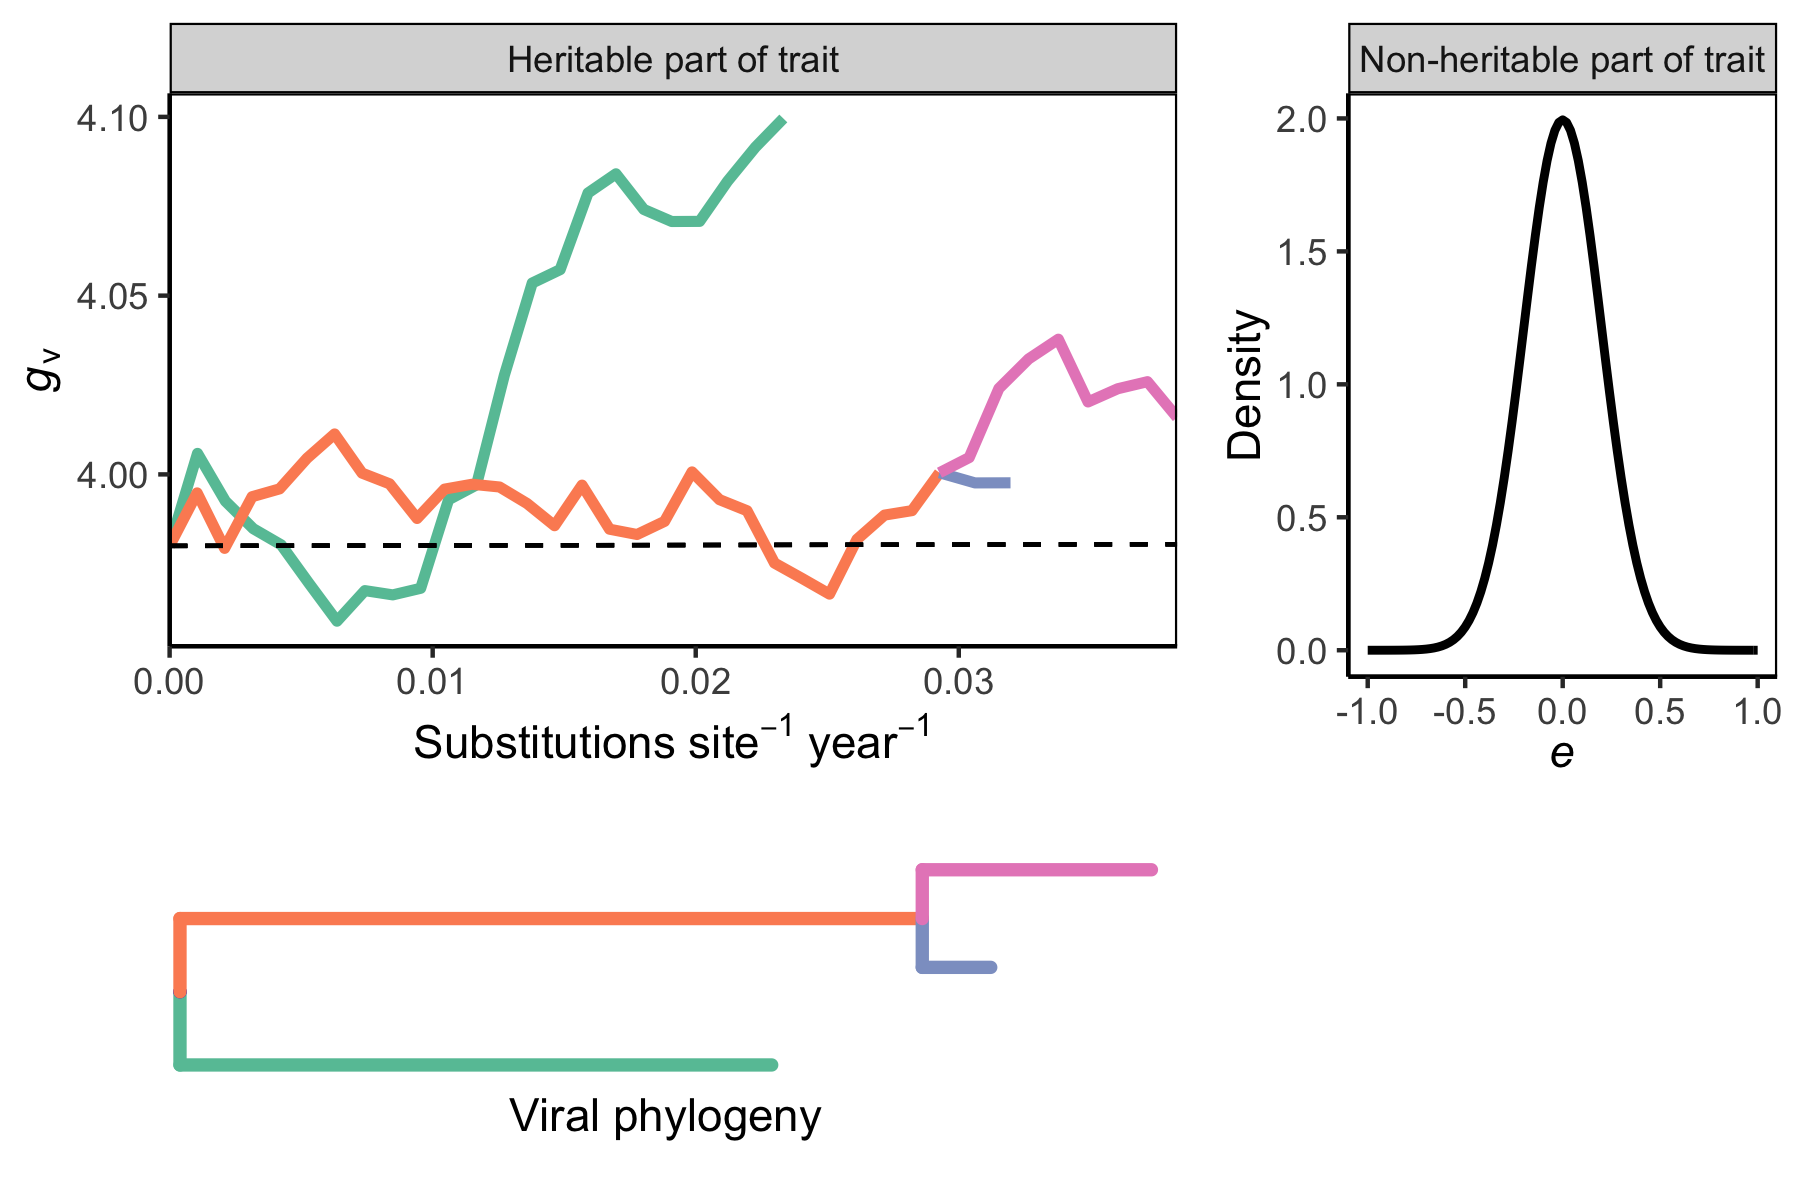
\includegraphics[width=0.75\linewidth]{figures/model_figure}
		\caption{The POUMM statistical model for the spVL trait. (A) shows how the pathogen effect on spVL, $g_v$, evolves according to an OU process along (C) the pathogen phylogeny. The dashed line in (A) shows the expected value of the trait at each point in time under the model. (B) shows that the non-pathogen effect on spVL, $e$, is modeled as a Gaussian random variable. Each tip on the phylogeny corresponds to a sampled individual with an independent non-pathogen-effect drawn from the distribution shown in (B).}
		\label{fig:spVLModel}
	\end{center}
\end{figure}

\subsection{Estimating and removing the virus-determined part of spVL}

Given the assumptions of the POUMM, we can derive a maximum-likelihood estimate for the virus-determined part of spVL for each individual in a cohort at the time they were sampled. Our goal is to estimate and remove this effect from measured spVL prior to GWAS. 

Let $\bm{g}_v(\bm{t})$ be a vector of $g_v$ values, one for each individual in the cohort. $\bm{t}$ are the sampling times of each individual relative to the root of the phylogeny. To simplify notation, we omit the $\bm{t}$ from here on. $\bm{g}_v$ is a realization of a Gaussian random vector $\bm{G_v} \sim \mathcal{N}\big(\bm{\mu}_{OU}, \boldsymbol{\Sigma}_{OU}\big)$. The expectation $\bm{\mu}_{OU}$ is defined by equation \ref{eq:OUmean}, the diagonal elements of the covariance matrix $\boldsymbol{\Sigma}_{OU}$ are defined by equation \ref{eq:OUVar}, and the off-diagonal elements of $\boldsymbol{\Sigma}_{OU}$ by equation \ref{eq:OUcov}. 

Similarly, let $\bm{e}$ be a vector of the environmental part of spVL for each individual.  $\bm{e}$ is a realization of a Gaussian random vector $\bm{E} \sim \mathcal{N}\big(\bm{0}, \boldsymbol{\Sigma}_E\big)$, where $\boldsymbol{\Sigma}_E$ is a diagonal matrix with diagonal elements equal to $\sigma^2_e$.

Considering that $\bm{G_v}$ and $\bm{E}$ are independent random vectors and that their realizations $\bm{g}_v$ and $\bm{e}$ must sum together to equal the observed spVL values $\bm{z}$, we can write the following proportionality for the joint probability density of $\bm{g}_v$ and $\bm{e}$:
\begin{equation}
	f\big(\bm{g}_v, \bm{e}\big) \propto \mathcal{N}\big(\bm{g}_v; \bm{\mu}_{G}, \boldsymbol{\Sigma}_G\big)
	\label{eq:pdfGprop}
\end{equation} 

where the expected value of $\bm{g}_v$ and the covariance matrix $\boldsymbol{\Sigma}_G$ are defined as:
\begin{align}
	Exp(\bm{g}_v) = \bm{\mu}_{G} &=  \boldsymbol{\Sigma}_G\big(\boldsymbol{\Sigma}_{OU}^{-1}\bm{\mu}_{OU} + \boldsymbol{\Sigma}_E^{-1} \bm{z}\big) \label{eq:MuG}\\
	\boldsymbol{\Sigma}_G &= \big(\boldsymbol{\Sigma}_{OU}^{-1} + \boldsymbol{\Sigma}_E^{-1}\big)^{-1} \label{eq:SigmaG}
\end{align}

\begin{proof}
	\begin{align}\label{eq:pdfG}
	\begin{split}
		f\big(\bm{g}_v,\ \bm{e}\big) &= f\big(\bm{g}_v|\ \bm{e}\big) \times f\big(\bm{e}\big) \\
	&= f\big(\bm{g}_v\big) \times f\big(\bm{e}\big) \\
	&= \mathcal{N}\big(\bm{g}_v;\ \bm{\mu}_{OU}, \mathbf{\Sigma}_{OU}\big) \times \mathcal{N}\big(\bm{e};\ \bm{0}, \mathbf{\Sigma}_E\big) \\
	&= \mathcal{N}\big(\bm{g}_v;\ \bm{\mu}_{OU}, \mathbf{\Sigma}_{OU}\big) \times \mathcal{N}\big(\bm{z} - \bm{g}_v;\ \bm{0}, \mathbf{\Sigma}_E\big) \\
	&= \mathcal{N}\big(\bm{g}_v;\ \bm{\mu}_{OU}, \mathbf{\Sigma}_{OU}\big) \times \mathcal{N}\big(\bm{g}_v;\ \bm{z}, \mathbf{\Sigma}_e\big)
	\end{split}
\end{align}
	
	Equations \ref{eq:MuG} and \ref{eq:SigmaG} follow from eq. \ref{eq:pdfG} and eq. 371, p. 42, section 8.1.8 ``Product of Gaussian densities'' in \citet{Petersen2012}.
\end{proof}

Importantly, equation \ref{eq:MuG} is the maximum likelihood estimate for $\bm{g}_v$, the viral part of spVL, taking into account all available information - the viral phylogeny, the inferred POUMM parameters, and measured spVL values. This estimator is an inverse-variance weighted average of information from the POUMM evolutionary model ($\bm{\mu}_{OU}$) and measured spVL ($\bm{z}$). Intuitively, the estimate for $g_v$ is closer to measured spVL if spVL is not very heritable, and is closer to the expected value under the POUMM if spVL is highly heritable. 

Given that we have an estimate for $\bm{g}_v$, we can finally estimate $\bm{e}$, representing the spVL value with viral effects removed: 
\begin{equation}
	\hat{\bm{e}} = \bm{z} - Exp(\bm{g}_v)
	\label{eq:EHat}
\end{equation}

\subsection{A new infectious disease GWAS framework}

We propose that by estimating and removing spVL variability due to the pathogen we can better measure the direct effects of human genetic variants on spVL. Our proposed framework is as follows:

\begin{enumerate}
	\item Sample host genotypes, host trait values, and pathogen genetic sequences from a cohort.
	\item Construct a pathogen phylogeny using the pathogen genetic sequences.
	\item Fit the POUMM to the trait values and the phylogeny. This produces estimates for parameters $g_0, \alpha, \theta, \sigma,\text{ and }\sigma_e$.
	\item Generate maximum-likelihood estimates for the pathogen-determined and environmental parts of the trait using equations \ref{eq:MuG} and \ref{eq:EHat}.
	\item Perform GWAS, using the estimated environmental part of the trait as the response variable instead of raw trait values. 
\end{enumerate}

\section{Results}

\subsection{Simulation study}

To test the theoretical best-case performance of our framework, we simulated data under the POUMM. Figure \ref{fig:sim-design} shows the simulation scheme and table \ref{tab:sim-params} gives the value or expression used for each parameter.

\subsubsection{Estimator accuracy}

First, we evaluated estimator accuracy with respect to $\bm{g}_h$, the sum of additive host genetic effects. This would be the ideal GWAS response variable to identify direct host determinants of spVL. We compute the accuracy of our proposed GWAS endpoint $\bm{\hat{e}}$ and the typical GWAS endpoint, measured spVL, using root mean squared error (RMSE). In our simulations we expect (scaled) measured spVL, $\bm{z} - \bar{\bm{z}}$, where $\bar{\bm{z}}$ is the average spVL, to be Gaussian distributed around $\bm{g}_h$ with variance equal to $\sigma^2_e + \sigma^2_{g_v} \approx 0.55$ (see table \ref{tab:sim-params} for simulation parameters). This should yield an RMSE of $\approx$ 0.74 for $\bm{z} - \bar{\bm{z}}$ as an estimate of $\bm{e}$, which matches simulation results (figure \ref{fig:simulationResults}A, scaled spVL). By incorporating information from the viral phylogenetic tree in calculating $\bm{\hat{e}}$, we were better able to estimate $\bm{e}$. The greatest improvement was possible in simulation scenarios in which spVL was highly heritable, meaning the virus contributed a great deal of variability to spVL. Estimates were also better in scenarios with lower selection strength since the correlation in $g_v$ among related tips is higher when $g_v$ can drift further from the long-term optimum and the stochastic fluctuations characterized by $\sigma$ are correspondingly lower to maintain the same viral genetic variance $\sigma^2_{g_v}$ and the same broad-sense heritability $H^2$.

\subsubsection{Theoretical GWAS improvement}

Next, we characterize the evolutionary scenarios in which our framework improves GWAS power. More accurate estimation of the non-viral part of spVL does not guarantee improved GWAS power. For example, if the viral part of spVL were constant across all viruses, association results (significance and effect size) would not be effected by a viral contribution to the trait. To determine under what evolutionary scenarios our method can improve GWAS power, we performed GWAS on the simulated data. Under our simulation set-up a standard GWAS would have $\approx$ 30\% power to detect a host variant explaining 1.25\% of the variability in spVL. This matches simulation results (figure \ref{fig:simulationResults}B, scaled spVL). Using our proposed framework, we were able to improve GWAS power in simulated scenarios with selection strength $<$ 10-20 time$^{-1}$ and spVL heritability $>$ 35-45\% (figure \ref{fig:simulationResults}B, $\bm{\hat{e}}$). If were were able to perfectly estimate $\bm{e}$, GWAS power would increase across all values of selection strength so long as the trait is highly heritable (figure \ref{fig:simulationResults}, $\bm{e}$). In summary, we show it is theoretically possible to improve GWAS power for heritable infectious disease traits by removing an estimated pathogen-determined effect.

\begin{figure}[H]
	\begin{center}
		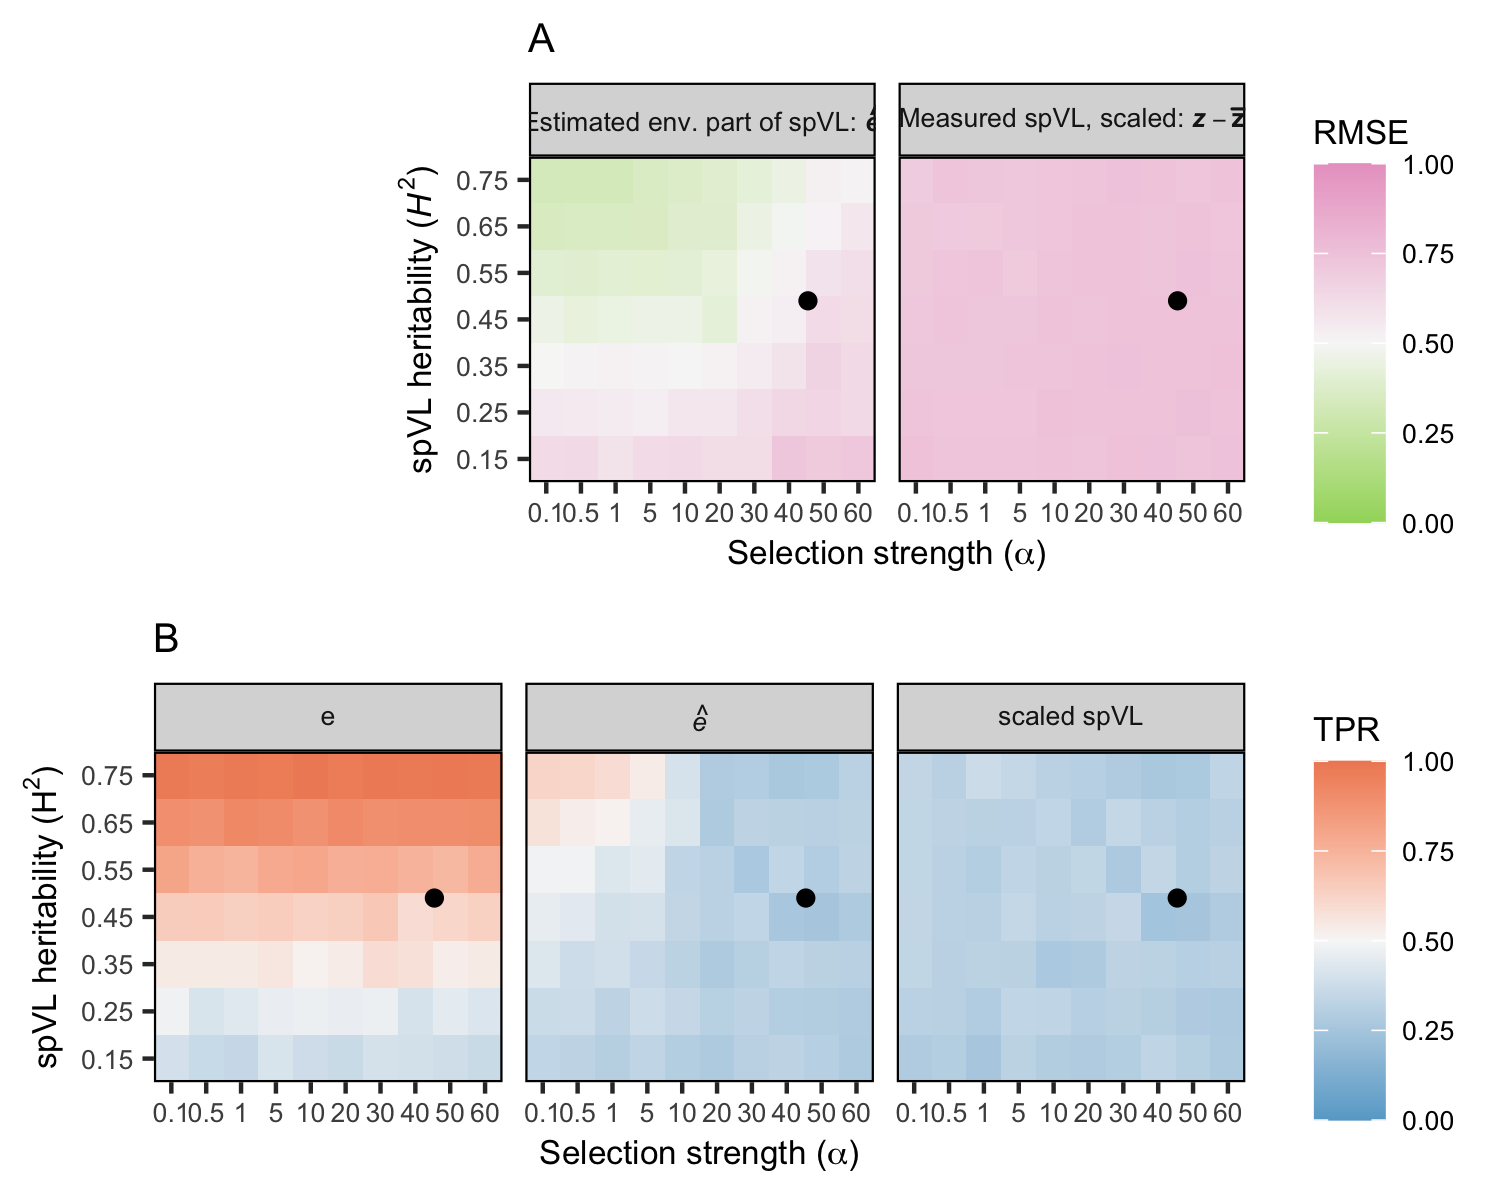
\includegraphics[width=0.75\linewidth]{figures/simulation_results}
		\caption{Results from the simulation study. We simulated pathogen and non-pathogen (host \& environmental) effects on the spVL trait under the POUMM with different trait heritability values (y-axis) and selection strengths (x-axis). For each simulated dataset, we applied our method to estimate the non-pathogen effects and performed GWAS using these estimates. (A) shows how well we can estimate the host effect using our method (left side) compared to just the scaled trait value (right side). (B) shows how GWAS can theoretically be improved by using the true (normally unknown) non-pathogen effects on spVL (left). It can still be improved in certain scenarios using our estimate for this value (middle) compared to the current standard - using just the (scaled) trait value (right). Tile color represents the average value over 20 simulated datasets of 500 samples for each heritability and selection strength value. The black point represents our estimates for the heritability and selection strength of spVL based on Swiss data. RMSE = Root mean square error, TPR = True positive rate.}
		% (RMSE) with respect to simulated values for the host part of spVL ($\bm{{g_h}}$) as a function of spVL trait heritability and selection strength on the trait. The left plot is for the POUMM-based estimate of the non-pathogen part of the trait ($\bm{\hat{e}}$) and the right plot is for the raw trait value scaled by the mean trait value, such that it is centered at zero ($\bm{z} - \bm{\bar{z}}$). (B) True positive rate (TPR) in GWAS performed using true (simulated) values for the non-pathogen part of the trait ($\bm{e}$), the POUMM-based estimate for the non-pathogen part of the trait ($\bm{\hat{e}}$), and the raw trait value scaled by the mean trait value ($\bm{z} - \bm{\bar{z}}$). The color of each plot tile in (A) and (B) represents the average value over 20 simulated datasets of 500 samples. The black point shows our estimates for the heritability of and selection strength on the spVL trait based on Swiss data.}
		\label{fig:simulationResults}
	\end{center}
\end{figure}

\subsection{GWAS on the Swiss HIV Cohort}

Finally, we demonstrate our framework on empirical data from the Swiss HIV Cohort Study (SHCS). In the ``standard GWAS" we followed a typical GWAS methodology,  i.e. regressing measured spVL ($\bm{z}$) on variant dosage for each sampled host genetic variant. In the ``GWAS with phylogenetic correction", we use our proposed framework, i.e. regressing the estimated environmental part of spVL ($\bm{\hat{e}}$) on variant dosage. In agreement with previous GWAS for host genetic determinants of spVL, the top associations were in the MHC and \emph{CCR5} regions for both GWAS (figure \ref{fig:gwas-results}). 

\begin{figure}[H]
	\begin{center}
		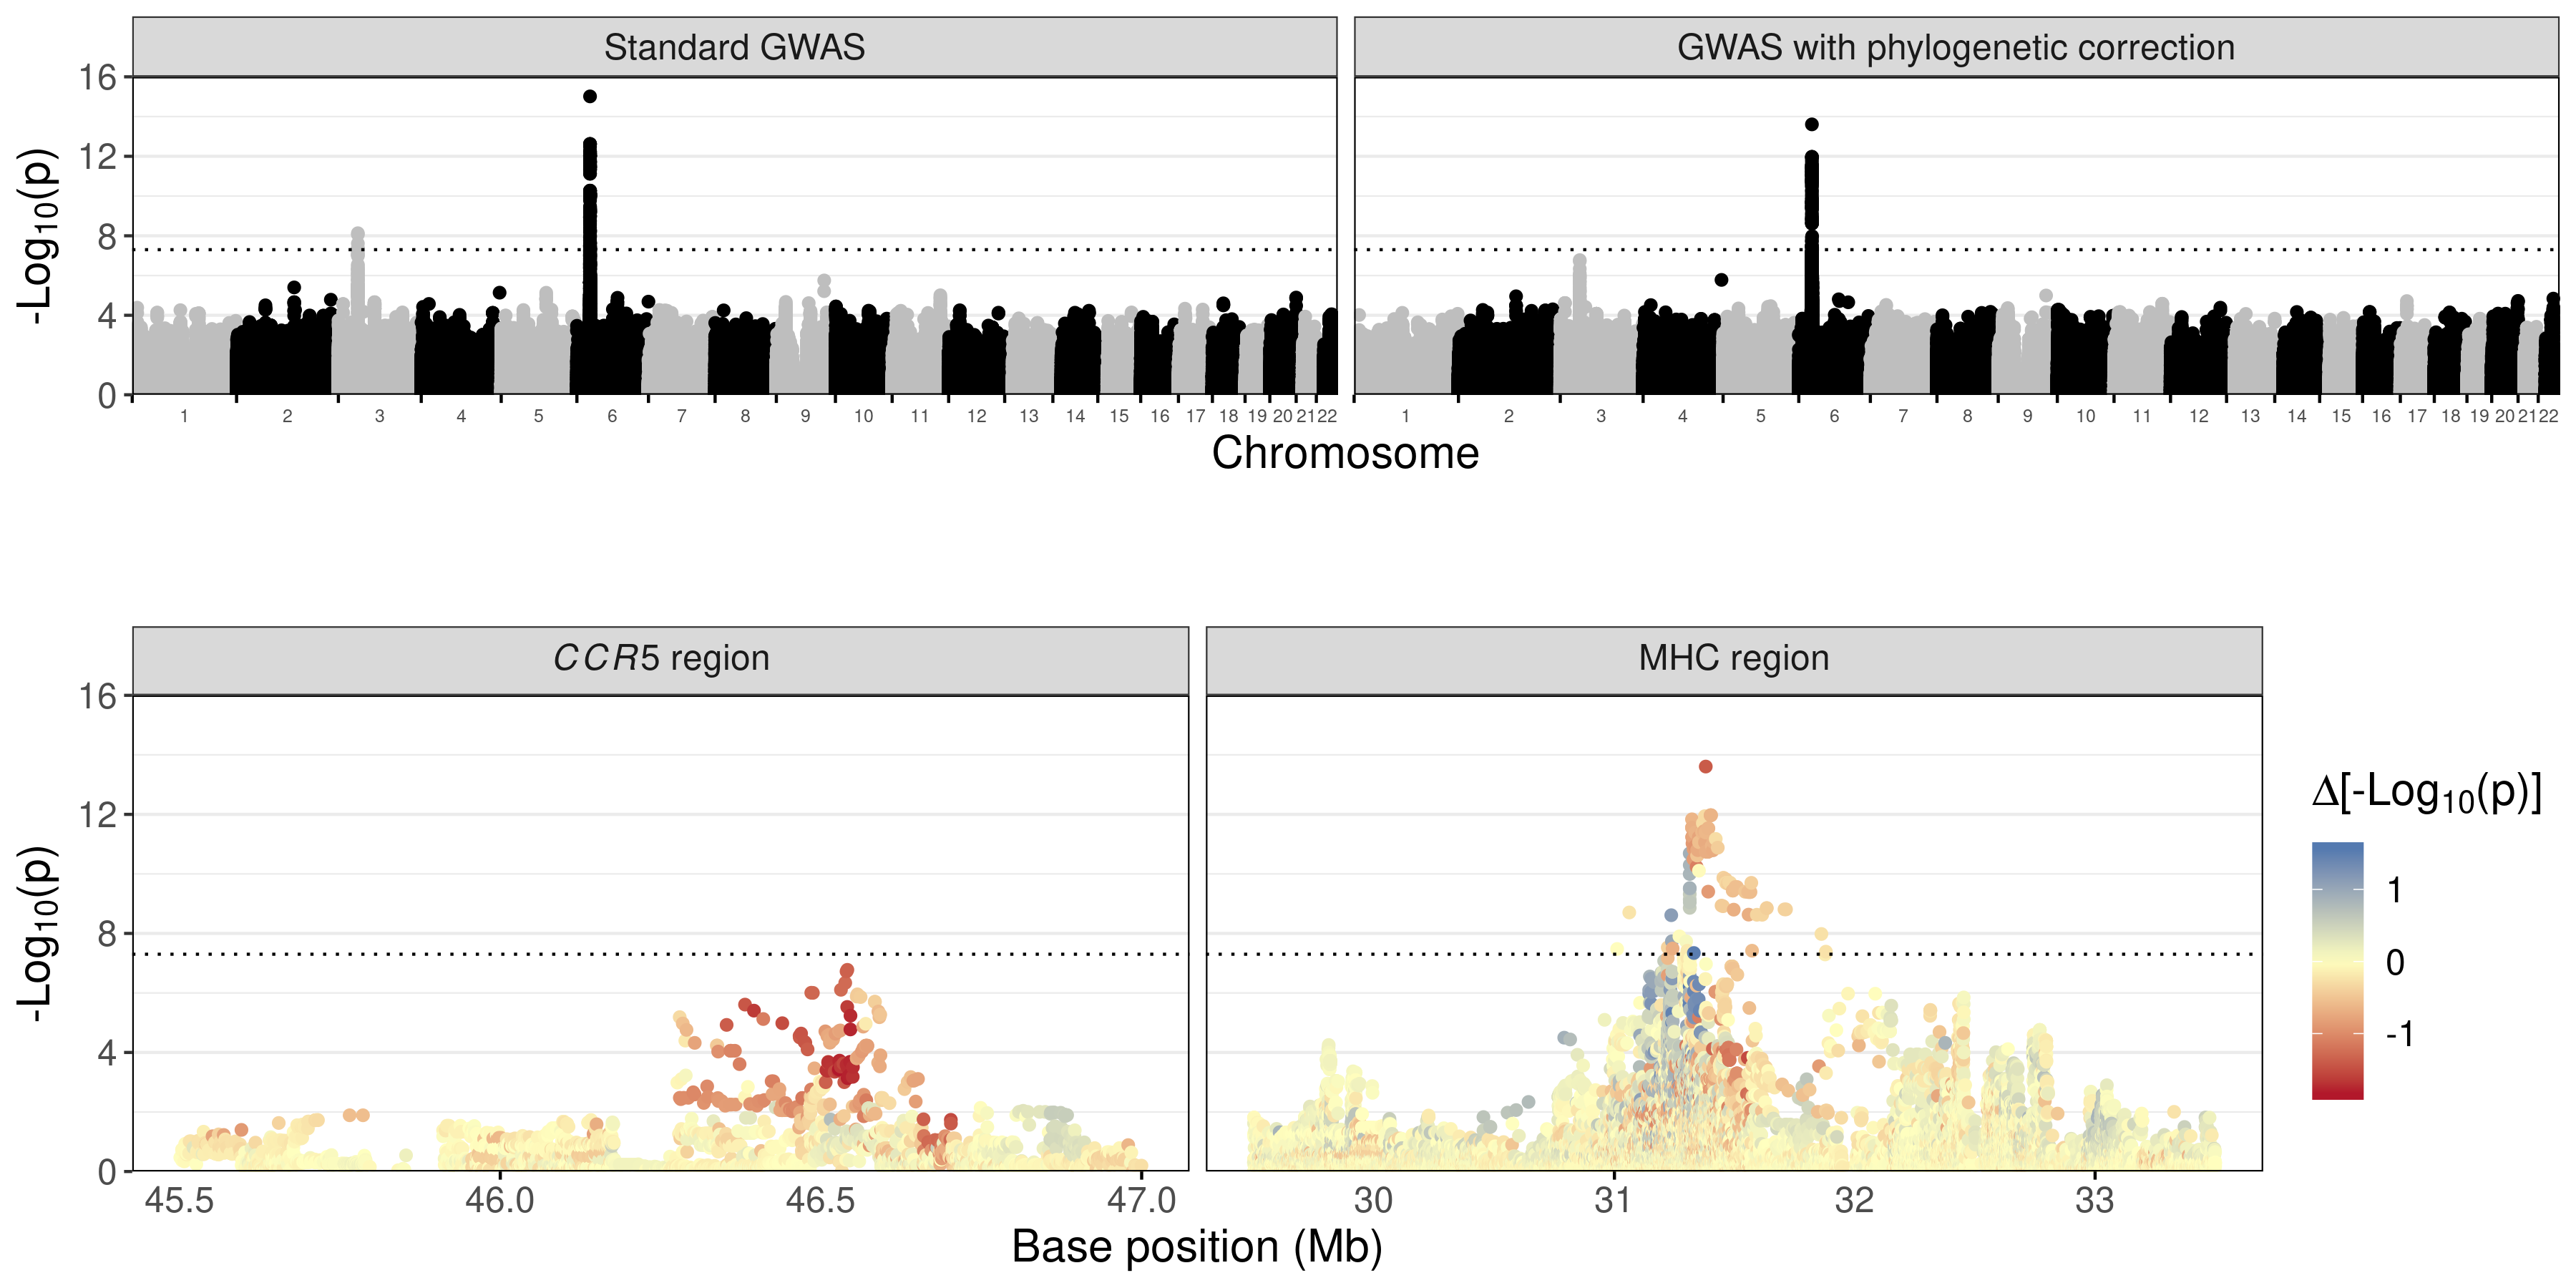
\includegraphics[width=\linewidth]{figures_archived/200207_gwas_results}
		\caption{Association results for standard GWAS and GWAS with a phylogenetic correction applied to the same data for HIV-1 set-point viral load. The pullout plots give regional association results from the GWAS with phylogenetic correction in the \emph{CCR5} region (positions 45.4 - 47Mb on chromosome 3) and the MHC region (positions 29.5 - 33.5Mb on chromosome 6). Base positions are with reference to genome build GRCh37. The color scale in the regional association plot is the difference in -log$_{10}$ p-value between the GWAS with phylogenetic correction and the standard GWAS. Red color means the phylogenetic correction decreased variant significance and blue color means the phylogenetic correction increased variant significance. The dashed lines show genome-wide significance (p-value = 5x10$^{-8}$).}
		\label{fig:gwas-results}
	\end{center}
\end{figure}

The overall distribution of p-values did not change noticeably between the standard GWAS and the GWAS with a phylogenetic correction (figure \ref{fig:qq-plots}). In the \emph{CCR5} and MHC regions, most variants decreased in significance in the GWAS with phylogenetic correction. However, the top-associated variants were constant between analyses. rs112243036 was most significant in the MHC, with a standard GWAS p-value of 9.7x10$^{-16}$ and corrected GWAS p-value of 2.5x10$^{-14}$. In the \emph{CCR5} region, rs7430431 was most significant, with a standard GWAS p-value of 7.4x10$^{-9}$ and a corrected GWAS p-value of 1.7x10$^{-7}$. Some variants in the MHC did increase in significance with a phylogenetic correction. For example, SNP rs9265880 had the greatest increase in significance from a p-value of 2.2x10$^{-5}$ in the standard GWAS to 6x10$^{-7}$ in the GWAS with phylogenetic correction. 

The top-associated SNPs from the \citet{McLaren2015} paper were excluded from the main analysis because of too-high missing rates (3\% for rs1015164 and 4\% for rs59440261). In order to directly compare our results with \citet{McLaren2015}, we ran an additional GWAS for these two SNPs anyways. Both SNPs became less significant with phylogenetic correction (table \ref{tab:comp-gwas}).

Again following the procedure of \citet{McLaren2015}, we imputed common HLA genotypes to more finely map association signals in the MHC region. Some HLA alleles also became more significant with a phylogenetic correction (table \ref{tab:lim-mclaren-comparison}).

\begin{table}[H]
	\begin{center}
		\begin{tabular}{p{1cm}p{2cm}p{2.5cm}p{1cm}p{2cm}p{1cm}p{2cm}} % {lrrrrrr} {llclcccc}
			\hline
			& & McLaren et al.  & \multicolumn{2}{l}{Standard GWAS } & \multicolumn{2}{l}{GWAS with phylogenetic correction} \\ 
			\hline
			Region & Variant & p-value & Beta & p-value & Beta & p-value \\
			\hline
			MHC & rs59440261 & 2.0 x 10$^{-83}$ & -0.414 & 1.6x10$^{-11}$ & -0.229 & 1.2x10$^{-10}$ \\
			\emph{CCR5} & rs1015164 & 1.5 x 10$^{-19}$ & 0.148 & 1.3x10$^{-6}$ & 0.073 & 3.2x10$^{-5}$ \\			
			\hline
		\end{tabular}
		\caption{Top association results from \citet{McLaren2015} compared to association results in the current study.}
		\label{tab:comp-gwas}
	\end{center}
\end{table}

\begin{table}[H]
	\begin{center}
	\begin{tabular} {p{3cm}p{1cm}p{2cm}p{1cm}p{2cm}p{1cm}p{2cm}} % {lrrrrrr}
		\hline
		 & \multicolumn{2}{l}{McLaren et al.}  & \multicolumn{2}{l}{Standard GWAS } & \multicolumn{2}{l}{GWAS with phylogenetic correction} \\ 
		 \hline
		Allele & Beta & p-value & Beta & p-value & Beta & p-value \\
		\hline	
		HLA-B*57:01 & -0.840 & $2.69 \times 10^{-86}$ & -0.479 & $1.11 \times 10^{-12}$ & -0.268 & $5.43 \times 10^{-12}$ \\ 
		\rowcolor{Gray}
		HLA-C*06:02 & -0.436 & $7.32 \times 10^{-50}$ & -0.173 & $1.10 \times 10^{-4}$ & -0.107 & $3.15 \times 10^{-5}$ \\ 
		HLA-B*27:05 & -0.417 & $4.32 \times 10^{-20}$ & -0.244 & $9.59 \times 10^{-4}$ & -0.122 & $4.40 \times 10^{-3}$ \\ 
		\rowcolor{Gray}
		HLA-C*07:01 & 0.195 & $1.86 \times 10^{-14}$ & 0.129 & $7.55 \times 10^{-3}$ & 0.086 & $1.99 \times 10^{-3}$ \\ 
		HLA-C*07:02 & 0.194 & $3.75 \times 10^{-13}$ & 0.095 & $3.02 \times 10^{-2}$ & 0.052 & $3.98 \times 10^{-2}$ \\ 
		HLA-B*07:02 & 0.200 & $5.17 \times 10^{-13}$ & 0.129 & $5.29 \times 10^{-3}$ & 0.072 & $7.06 \times 10^{-3}$ \\ 
		\rowcolor{Gray}
		HLA-B*08:01 & 0.206 & $2.94 \times 10^{-11}$ & -0.009 & $9.20 \times 10^{-1}$ & 0.015 & $7.75 \times 10^{-1}$ \\ 
		\rowcolor{Gray}
		HLA-C*08:02 & -0.307 & $8.76 \times 10^{-11}$ & 0.324 & $8.55 \times 10^{-1}$ & 0.400 & $6.95 \times 10^{-1}$ \\ 
		HLA-C*04:01 & 0.183 & $9.07 \times 10^{-11}$ & 0.124 & $3.04 \times 10^{-3}$ & 0.058 & $1.67 \times 10^{-2}$ \\ 
		\rowcolor{Gray}
		HLA-B*13:02 & -0.346 & $3.70 \times 10^{-10}$ & -0.188 & $1.03 \times 10^{-2}$ & -0.112 & $7.90 \times 10^{-3}$ \\ 
		\rowcolor{Gray}
		HLA-B*14:02 & -0.318 & $2.10 \times 10^{-9}$ & 0.067 & $8.12 \times 10^{-1}$ & 0.118 & $4.71 \times 10^{-1}$ \\ 
		\rowcolor{Gray}
		HLA-C*12:02 & -0.478 & $4.02 \times 10^{-8}$ & 0.111 & $7.63 \times 10^{-1}$ & 0.094 & $6.58 \times 10^{-1}$ \\
		\hline
	\end{tabular}
	\caption{Association results for common class I HLA alleles ranked by p-value from the GWAS by \citet{McLaren2015} compared to results from the current study. The table is truncated to show only alleles that reached genome-wide significance in the McLaren et al. study. The full table is available in the supplement (table \ref{tab:full-mclaren-comparison}). Grey rows are alleles that increased in significance with a phylogenetic correction.}
	\label{tab:lim-mclaren-comparison}
	\end{center}
\end{table}



\section{Discussion}
\begin{itemize}
	\item From the field of phylogenetic comparative methods there are several methods to account for non-independence among samples related by an underlying phylogeny (e.g. independent contrasts, phylogenetic generalized least squares). Compared to these methods, our method is nice for GWAS because we do not change the association model itself, instead we just adjust the trait values prior to association testing.
\end{itemize}

%\begin{itemize}
%	\item Compare inferred POUMM parameters to previous studies \parencite{Mitov2018, Bertels2018}
%	\item Standard GWAS highlights previously identified regions associated with spVL: $CCR5$ and MHC
%	\item We expect non-viral only GWAS to increase signals of association in $CCR5$ (because noise in spVL from the virus reduced) and decrease signals of association in MHC (because viral mutations mediate MHC effects). It \emph{seems} like the results support these hypotheses, but I am waiting on POUMM parameter estimates from a longer MCMC run.
%	\item The phylogenetic correction to GWAS leads to the biggest p-value changes in the $CCR5$ and MHC regions
%	\item SNPs near the FUT1 gene (on chromosome 6, highlighted as one of the top-20 p-value changes in the first pipeline run) increased in significance, and the Lewis-X antigen produced by this gene is known to play a role in early HIV infection \cite{Naarding2005}.
%	\item Address method caveats: 
%	\begin{itemize}
%		\item We don't model virus-host interaction effects
%		\item We don't account for uncertainty in non-viral component of spVL estimates
%	\end{itemize}
%	\item Implications for future research: what other infectious disease traits are heritable?
%\end{itemize}

\section{Methods}

\subsection{Simulation model}

Whenever possible, we tried to parameterize our simulation model for spVL using empirical data. We set the total variance in spVL to 0.73 log copies$^2$ mL$^{-2}$ based on UK cohort data \parencite{Mitov2018}. After allotting 25\% of this variance to the host part of spVL $g_h$ (following \citealt{McLaren2015}), we partitioned the remaining variance between the viral part $g_v$ and the environmental part $\epsilon$ in different ratios to assess estimator performance across a range of spVL heritabilities. $g_h$ was simulated as the sum of contributions from 20 causal host genetic variants, 10 of which had an effect size of 0.2 log copies mL$^{-1}$ and 10 of which had an effect size of -0.2 log copies mL$^{-1}$. Host genetic variants were generated from a binomial distribution with probability $p$ calculated such that $g_h$ had the appropriate variance (see table \ref{tab:sim-params}). We generated a random viral phylogeny with branch lengths on the same time scale as a previously inferred UK cohort HIV tree \parencite{Hodcroft2014} using the R package ape \parencite{Paradis2018}. $g_v$ was simulated by running an OU process along the phylogeny using the R package POUMM \parencite{Mitov2017a-POUMM} and sampling values at the tips. For the OU parameters $\theta$ and $g_{0}$ we used 4.5 log copies mL$^{-1}$, similar to values previously inferred for HIV (table \ref{tab:POUMMparams}). To assess our estimator's performance under a range of evolutionary scenarios, we co-varied the OU parameters for selection strength, $\alpha$, and intensity of random fluctuations, $\sigma$, so that different proportions of the variability in $g_v$ were attributable to selection and drift, respectively. Finally, the environmental component of spVL $\epsilon$ was generated from a normal distribution with mean 0.

\begin{table}[H]
	\begin{tabular}{p{1.5cm}ll} \toprule 
		Variable & Expression & Definition \\ \midrule 
		$\sigma^2_z$ &  0.73 log copies$^{2}$/mL$^{2}$ & total spVL variance \\ 
		$H^2_{\bar{t}}$ & varied & spVL viral heritability at $\bar{t}$ \\
		$\sigma^2_{g_h}$ & $\sigma_{g_h}^2 = 0.25*\sigma_z^2$ & variance in host part of spVL \\
		$\sigma^2_{g_v}(\bar{t})$ & $\sigma^2_{g_{v}}(\bar{t}) = H^2_{\bar{t}}*\sigma_z^2$ & variance in viral part of spVL at $\bar{t}$ \\ 
		$\sigma^2_{\epsilon}$ & $\sigma_{\epsilon}^2 = \sigma_z^2 - \sigma^2_{g_v} - \sigma^2_{g_h}$ & variance in environmental part of spVL \\ 
		$\bar{t}$ & 0.14 substitutions site$^{-1}$ yr$^{-1}$ & mean root-tip time in viral phylogeny \\ 
		$\bm{g}_v$ & $\bm{g}_v \sim Norm(\bm{\mu}_{OU}, \boldsymbol{\Sigma}_{OU})$ & viral part of spVL for all individuals \\ 
		$\theta$ & 4.5 log copies/mL & optimal spVL value \\
		$g_{0}$ & 4.5 log copies/mL & $g_v$ at the root of the phylogeny  \\ 
		$\alpha$ & varied & selection strength of OU process \\ 
		$\sigma$ & $\sigma = \sqrt{\frac{2\alpha\sigma^2_{g_{v}}(\bar{t})}{1 - exp(-2\alpha\bar{t})}}$ & time-unit standard deviation of OU process \\ 
		$\Psi$ & branch lengths $\sim Exp(\bar{t})$ & viral phylogeny \\ 
		$g_{h_i}$ & $g_{h_i} = \delta \sum_{j = 1}^{j = M/2}{G_{ij}} - \delta \sum_{j = M/2}^{j = M}{G_{ij}}$ & host part of spVL for individual $i$ \\ 
		$G_{N \times M}$ & $G_{ij} \sim Binom(2, p)\ \forall i \in {1...N}, \forall j \in {1...M}$ & host genotype matrix \\
		$p$ & $p = \frac{1}{2} - \sqrt{\frac{1}{4} - \frac{H_{\bar{t}}^2\sigma^2_z}{2\delta^2M}}$ &  host variant allele frequency \\ 
		$\delta$ & 0.2 & host variant effect size \\ 
		$M$ & 20 & number of causal host variants \\ 
		$\epsilon_i$ & $ \epsilon_i \sim Norm(0, \sigma^2_{\epsilon})$ & environmental part of spVL for individual $i$ \\ \bottomrule 
	\end{tabular}
	\caption{Simulation model parameters.}
	\label{tab:sim-params}
\end{table}

\subsection{Swiss HIV-1 data}

Genotypes, viral load measurements, and HIV-1 $pol$ gene sequences from HIV-1 positive individuals were all collected in the context of other studies by the Swiss HIV Cohort Study (SHCS, \citealt{Schoeni-Affolter2010}). 

We retained data from 1,396 individuals with non-recombinant subtype B $pol$ gene sequences of at least 750 characters, paired RNA measurements allowing for calculation of spVL, European ancestry, and not closely related to other individuals in the cohort (Table \ref{tab:sample-filtering}). Viral subtype was determined by the SHCS using the REGA HIV subtyping tool version 2.0 \parencite{DeOliveira2005}. We calculated spVL as the arithmetic mean of viral RNA measurements made prior to the start of antiretroviral treatment. Ancestry was determined by plotting individuals along the three primary axes of genotypic variation from a combined dataset of SHCS samples and HapMap populations (Figure \ref{fig:PCA}). Kinship was evaluated using PLINK version 2.00a2LM \parencite{Chang2015}; we used the --king-cutoff option to exclude one from each pair of individuals with a kinship coefficient $>$ 0.09375. 

For phylogenetic inference, we included the 1,396 subtype B sequences and 5 randomly chosen subtype A sequences from the SHCS as an outgroup. We used MUSCLE version 3.8.31 \parencite{edgar_muscle:_2004} to align the $pol$ sequences with --maxiters 3 and otherwise default settings. We trimmed the alignment to 1505 characters to standardize sequence lengths. We used IQ-TREE version 1.6.9 to construct an approximate maximum likelihood tree with -m GTR+F+R4 for a general time reversible substitution model with empirical base frequencies and four free substitution rate categories. Otherwise, we used the default IQ-TREE settings. After rooting the tree based on the subtype A samples, we removed the outgroup.

Initial host genotyping quality control and imputation were done by the SHCS. Subsequent genotyping quality control was performed using PLINK version 2.3 \parencite{Chang2015}. We used the options --maf 0.01, --geno 0.01, and --hwe 0.00005 to remove variants with minor allele frequency less than 0.01, missing call rate greater than 0.01, or Hardy-Weinberg equilibrium exact test p-value less than 5x10$^-5$. After quality filtering, approximately XXX million genetic variants from XXX individuals were retained for GWAS (Table \ref{tab:variant-filtering}). 

\subsection{POUMM parameter inference}

We used the R package POUMM version 2.1.6 \parencite{Mitov2017a-POUMM} to infer the POUMM parameters $g_0, \alpha, \theta, \sigma, \text{ and }\sigma_e$ from the approximate maximum-likelihood phylogeny and calculated spVL values. The Bayesian inference method implemented in this package requires specification of a prior distribution for each parameter. We used the same, broad prior distributions as in \citet{Mitov2018}, namely: $g_{0} \sim \mathcal{N}(4.5,\ 3)$, $\alpha \sim Exp(0.02)$, $\theta \sim \mathcal{N}(4.5,\ 3)$, $H^2_{\bar{t}} \sim \mathcal{U}(0,\ 1)$, and $\sigma^2_e \sim Exp(0.02)$. We ran two MCMC chains for 4x10$^6$ samples each with a target sample acceptance rate of 0.01 and a thinning interval of 1000. The first 2x10$^5$ samples of each chain were used for automatic adjustment of the MCMC proposal distribution. Inferred parameters, posterior distributions for inferred parameters, and MCMC trace plots are given in table \ref{tab:POUMM-parameters} and figure \ref{fig:poumm-fit}, respectively.

\subsection{Phylogenetic spVL correction}
We corrected calcualted spVL values using the method described in this paper. For each of the 1,396 individuals in our cohort, we estimated the viral part of spVL using equation \ref{eq:MuG} and the corresponding non-viral part using equation \ref{eq:EHat}. For the POUMM parameters $\alpha$, $\sigma$, $\theta$, and $\sigma_e$, we used the maximum posterior probability estimates generated as described above. 

\subsection{Association testing}
We performed two GWAS using the same genotype data. For the first ``standard GWAS" we used total calculated spVL ($\bm{z}$) as the dependent variable for association testing, replicating prior GWAS for host genetic determinants of spVL. For the second ``GWAS with phylogenetic correction" we replaced total spVL with the estimated non-viral component of spVL ($\hat{\bm{e}}$) as the dependent variable. Association testing was performed using a linear association model in PLINK version 2.3 \parencite{Chang2015} with sex and the top 5 principle components of host genetic variation included as covariates. The sex and principle components covariates were included to reduce residual variance in spVL and control for confounding from host population structure, respectively. Common HLA allele genotypes were imputed using the SNP2HLA pipeline \parencite{Jia2013a} with a reference panel of 124 individuals from the HapMap CEU population. Association tests for imputed HLA alleles were performed in the same way as for other variants. 

\section{Acknowledgments}

\begin{itemize}
	\item Thanks to Michael Landis, who shared a LaTeX template for graphical model drawing.
	\item Esposito Mauro and Alexandra Scherrer from the SHCS data center were especially helpful in retrieving data.
\end{itemize}


%Additional ideas for supplemental materials:
%\begin{itemize}
%	\item Table of genotype samples by project (genotyping chip, number of samples, spVL distribution)
%	\item Link to github with all the code used to run simulations and generate figures
%	\item Example spVL plots
%	\item simulated TPR plot annotated with actual inferred POUMM params
%	\item Simulation results with different parameterizations
%	\item Whole pipeline replicated with a stricter spVL definition (and correspondingly fewer samples)
%	\item Comparative QQ-plots from 1500 and standard GWAS
%	\item Proof of robustness of method to inferred tree
%\end{itemize}

\newpage
\section{Supplemental Material}
\beginsupplement

\subsection{Expected results from simulations}

Here we show the root mean square error (RMSE) of $\bm{z} - \bm{\bar{z}}$ as an estimate for $\bm{h}$ should be $\approx$ 0.74 in our simulation setup. First we write the expression for the RMSE:

\begin{equation}
    RMSE = \sqrt{\frac{\sum_i^N(z - \bar{z} - h)^2}{N}}
\end{equation}

Note that $z - \bar{z}$ differs from $h$ due to a viral effect and an environmental effect. So the term inside the square root equals the combined variance of these two effects:

\begin{equation}
    RMSE = \sqrt{\sigma^2_{g_v} + \sigma^2_\epsilon}
\end{equation}

We can calculate the variance due to these two effects because the total variance in spVL $\sigma^2_z$, and the fraction of the total variance due to host genetic effects, $\sigma^2_{g_h}$, are fixed parameters in our simulation setup.

\begin{equation}
\begin{split}
    \sigma^2_{g_h} + \sigma^2_{g_v} + \sigma^2_\epsilon = \sigma^2_z \\
    0.25 * \sigma^2_{z} + \sigma^2_{g_v} + \sigma^2_\epsilon = \sigma^2_z \\
    \sigma^2_{g_v} + \sigma^2_\epsilon = 0.75 * \sigma^2_z \\
    \sigma^2_{g_v} + \sigma^2_\epsilon = 0.75 * 0.73 \\
    \sigma^2_{g_v} + \sigma^2_\epsilon = 0.55
\end{split}
\end{equation}

Therefore, we can expect the RMSE for $\bm{z} - \bm{\bar{z}}$ as an estimate for $\bm{h}$ to be around $\sqrt{0.55} \approx 0.74$. 

\newpage

\begin{figure}[H]
	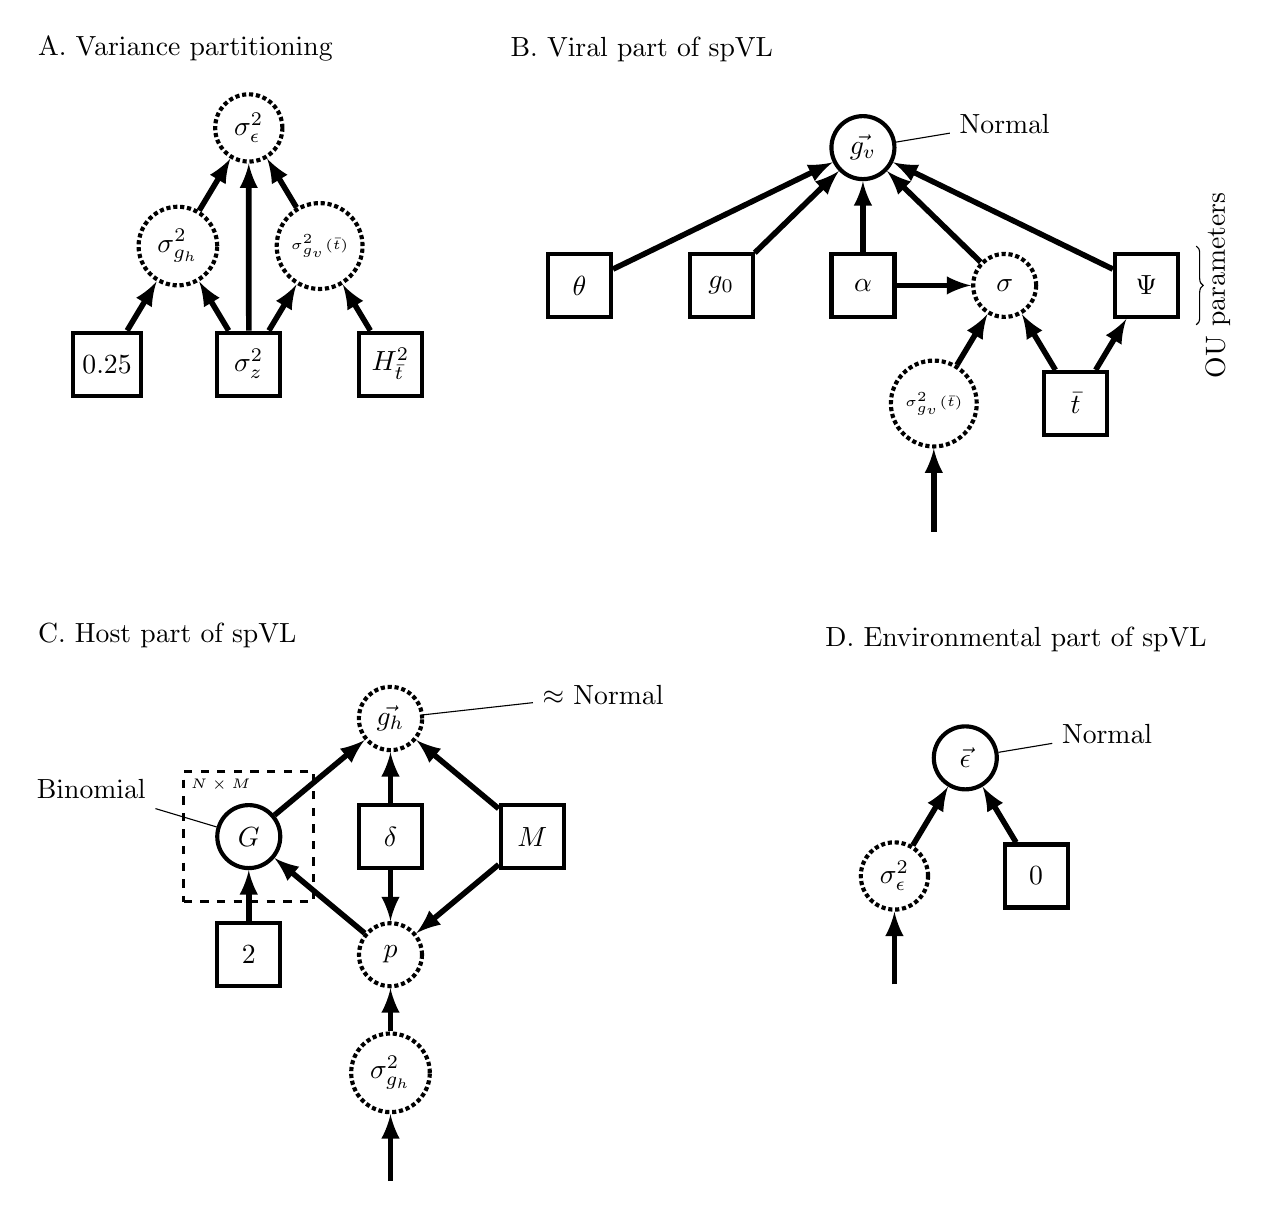
\begin{tikzpicture}
	
	% Variance 
	\begin{scope}[xshift = 0cm, yshift = 0cm]
	\node[anchor = west] (alabel) at (-1, 4) {A. Variance partitioning};
	\node[constnode] (H2h) at (0, 0) {0.25};
	\node[constnode] (varz) at ($(H2h) + (1.8, 0)$) {$\sigma^2_z$};
	\node[constnode] (H2) at ($(H2h) + (3.6, 0)$) {$H^2_{\bar{t}}$};
	\node[detnode] (varh) at ($(H2h) + (0.9, 1.5)$) {$\sigma^2_{g_h}$};
	\node[detnode] (varv) at ($(varz) + (0.9, 1.5)$) {\tiny $\sigma^2_{g_{v}}(\bar{t})$};
	\node[detnode] (vare) at ($(varh) + (0.9, 1.5)$) {$\sigma^2_{\epsilon}$};
	\draw[taro] (H2h) -- (varh);
	\draw[taro] (varz) -- (varh);
	\draw[taro] (varz) -- (varv);
	\draw[taro] (H2) -- (varv);
	\draw[taro] (varh) -- (vare);
	\draw[taro] (varv) -- (vare);
	\draw[taro] (varz) -- (vare);
	\end{scope}
	
	% Virus
	\begin{scope}[xshift = 6cm, yshift = -0.5cm]
	\node[anchor = west] (blabel) at (-1, 4.5) {B. Viral part of spVL};
	\node[constnode] (theta) at (0, 1.5) {$\theta$};
	\node[constnode] (g0) at (1.8, 1.5) {$g_{0}$};
	\node[constnode] (alpha) at (3.6, 1.5) {$\alpha$};
	\node[detnode] (sigma) at (5.4, 1.5) {$\sigma$};
	\node[constnode] (tree) at (7.2, 1.5) {$\Psi$};
	\node[detnode] (varv) at (3.6+0.9, 0) {\tiny $\sigma^2_{g_{v}}(\bar{t})$};
	\node[constnode] (tbar) at (3.6+0.9+1.8, 0) {$\bar{t}$};
	\node[snode] (v) at (3.6, 3.25) {$\vec{g_v}$};
	\draw[taro] (theta) -- (v);
	\draw[taro] (g0) -- (v);
	\draw[taro] (alpha) -- (v);
	\draw[taro] (sigma) -- (v);
	\draw[taro] (tree) -- (v);
	\draw[taro] (varv) -- (sigma);
	\draw[taro] (tbar) -- (sigma);
	\draw[taro] (tbar) -- (tree);
	\draw[taro] (alpha) -- (sigma);
	\node[white] (varpic) at (3.6+0.9, -1.75) {};
	\draw[taro] (varpic) -- (varv);
	\node (vdist) at ($(v) + (1.8, 0.3)$) {Normal};
	\draw (v) -- (vdist);
	\draw[decoration={brace, mirror, raise=18pt}, sloped, decorate] (7.2, 1.5 - .5) -- node[below = 18pt] {OU parameters} (7.2, 1.5 + .5);
	\end{scope}
	
	% Host 
	\begin{scope}[xshift = 0cm, yshift = -9cm]
	\node[anchor = west] (clabel) at (-1, 5.55) {C. Host part of spVL};
	\node[constnode] (d) at (1.8, 1.5) {2};
	\node[detnode] (p) at (3.6, 1.5) {$p$};
	\node[snode] (G) at (1.8, 3) {$G$};
	\node[rectangle, dashed, very thick, inner sep=4mm, draw=black!100, fit = (G) ] (Gplate) {};
	\node[anchor=north west, inner sep=3pt] at (Gplate.north west) {\tiny $N\times M$};
	\node[detnode] (varh) at (3.6, 0) {$\sigma^2_{g_h}$};
	\node[constnode] (delta) at (3.6, 3) {$\delta$};
	\node[detnode] (h) at (3.6, 4.5) {$\vec{g_h}$};
	\node[constnode] (M) at (5.4, 3) {$M$};
	\draw[taro] (d) -- (G);
	\draw[taro] (p) -- (G);
	\draw[taro] (varh) -- (p);
	\draw[taro] (delta) -- (p);
	\draw[taro] (M) -- (p);
	\draw[taro] (M) -- (h);
	\draw[taro] (delta) -- (h);
	\draw[taro] (G) -- (h);
	\node[white] (varpic) at (3.6, -1.5) {};
	\draw[taro] (varpic) -- (varh);
	\node (hdist) at ($(h) + (2.7, 0.3)$) {$\approx$ Normal};
	\draw (h) -- (hdist);
	\node (gdist) at ($(G) + (-2, 0.6)$) {Binomial};
	\draw (G) -- (gdist);
	\end{scope}
	
	% Environment
	\begin{scope}[xshift = 10cm, yshift = -6.5cm]
	\node[anchor = west] (dlabel) at (-1, 3) {D. Environmental part of spVL};
	\node[detnode] (vare) at (0, 0) {$\sigma^2_{\epsilon}$};
	\node[constnode] (zero) at ($(vare) + (1.8, 0)$) {0};
	\node[snode] (e) at ($(vare) + (1.8/2, 1.5)$) {$\vec{\epsilon}$};
	\draw[taro] (zero) -- (e);
	\draw[taro] (vare) -- (e);
	\node[white] (varpic) at (0, -1.5) {};
	\draw[taro] (varpic) -- (vare);
	\node (edist) at ($(e) + (1.8, 0.3)$) {Normal};
	\draw (e) -- (edist);
	\end{scope}
	
	\end{tikzpicture}
	\caption{A graphical representation of the simulation model. Variables in solid squares are constant in the simulation scheme, whereas variables in solid circles are realizations of random variables and variables in dashed circles are determined as a function of other variables. Arrows represent dependencies among variables and the dashed square represents repetition \parencite{Hohna2014}.}
	\label{fig:sim-design}
\end{figure}

\begin{figure}[H]
	\centering
		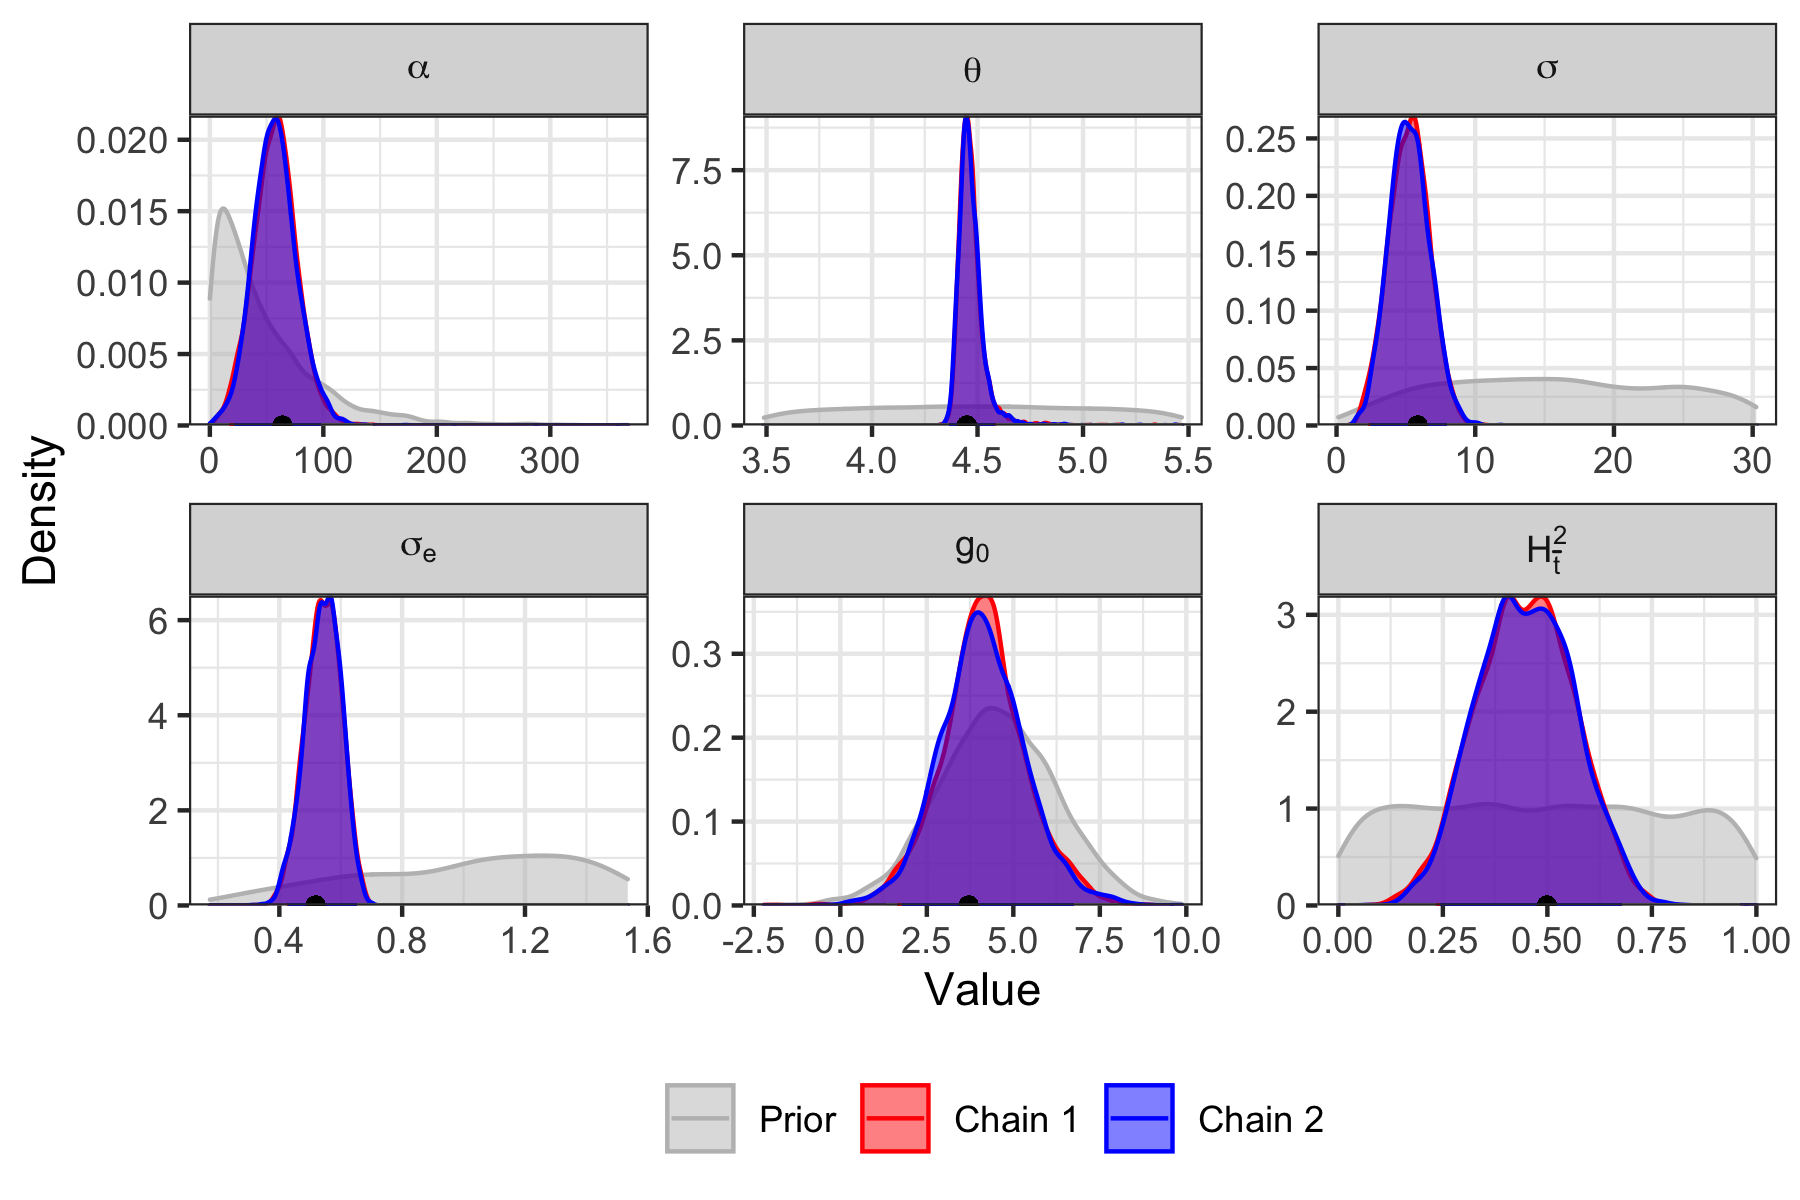
\includegraphics[width=\linewidth]{figures/poumm_parameter_estimates.png}
		\caption{Posterior distributions compared to the prior for POUMM parameter estimates based on Swiss data. We ran two different MCMC chains to ensure the estimates converged. The black point on the x-axis shows the posterior mean value, which was used to estimate the pathogen- and non-pathogen effects on spVL.}
\label{fig:poumm-parameters}
\end{figure}

\begin{figure}[H]
\begin{center}
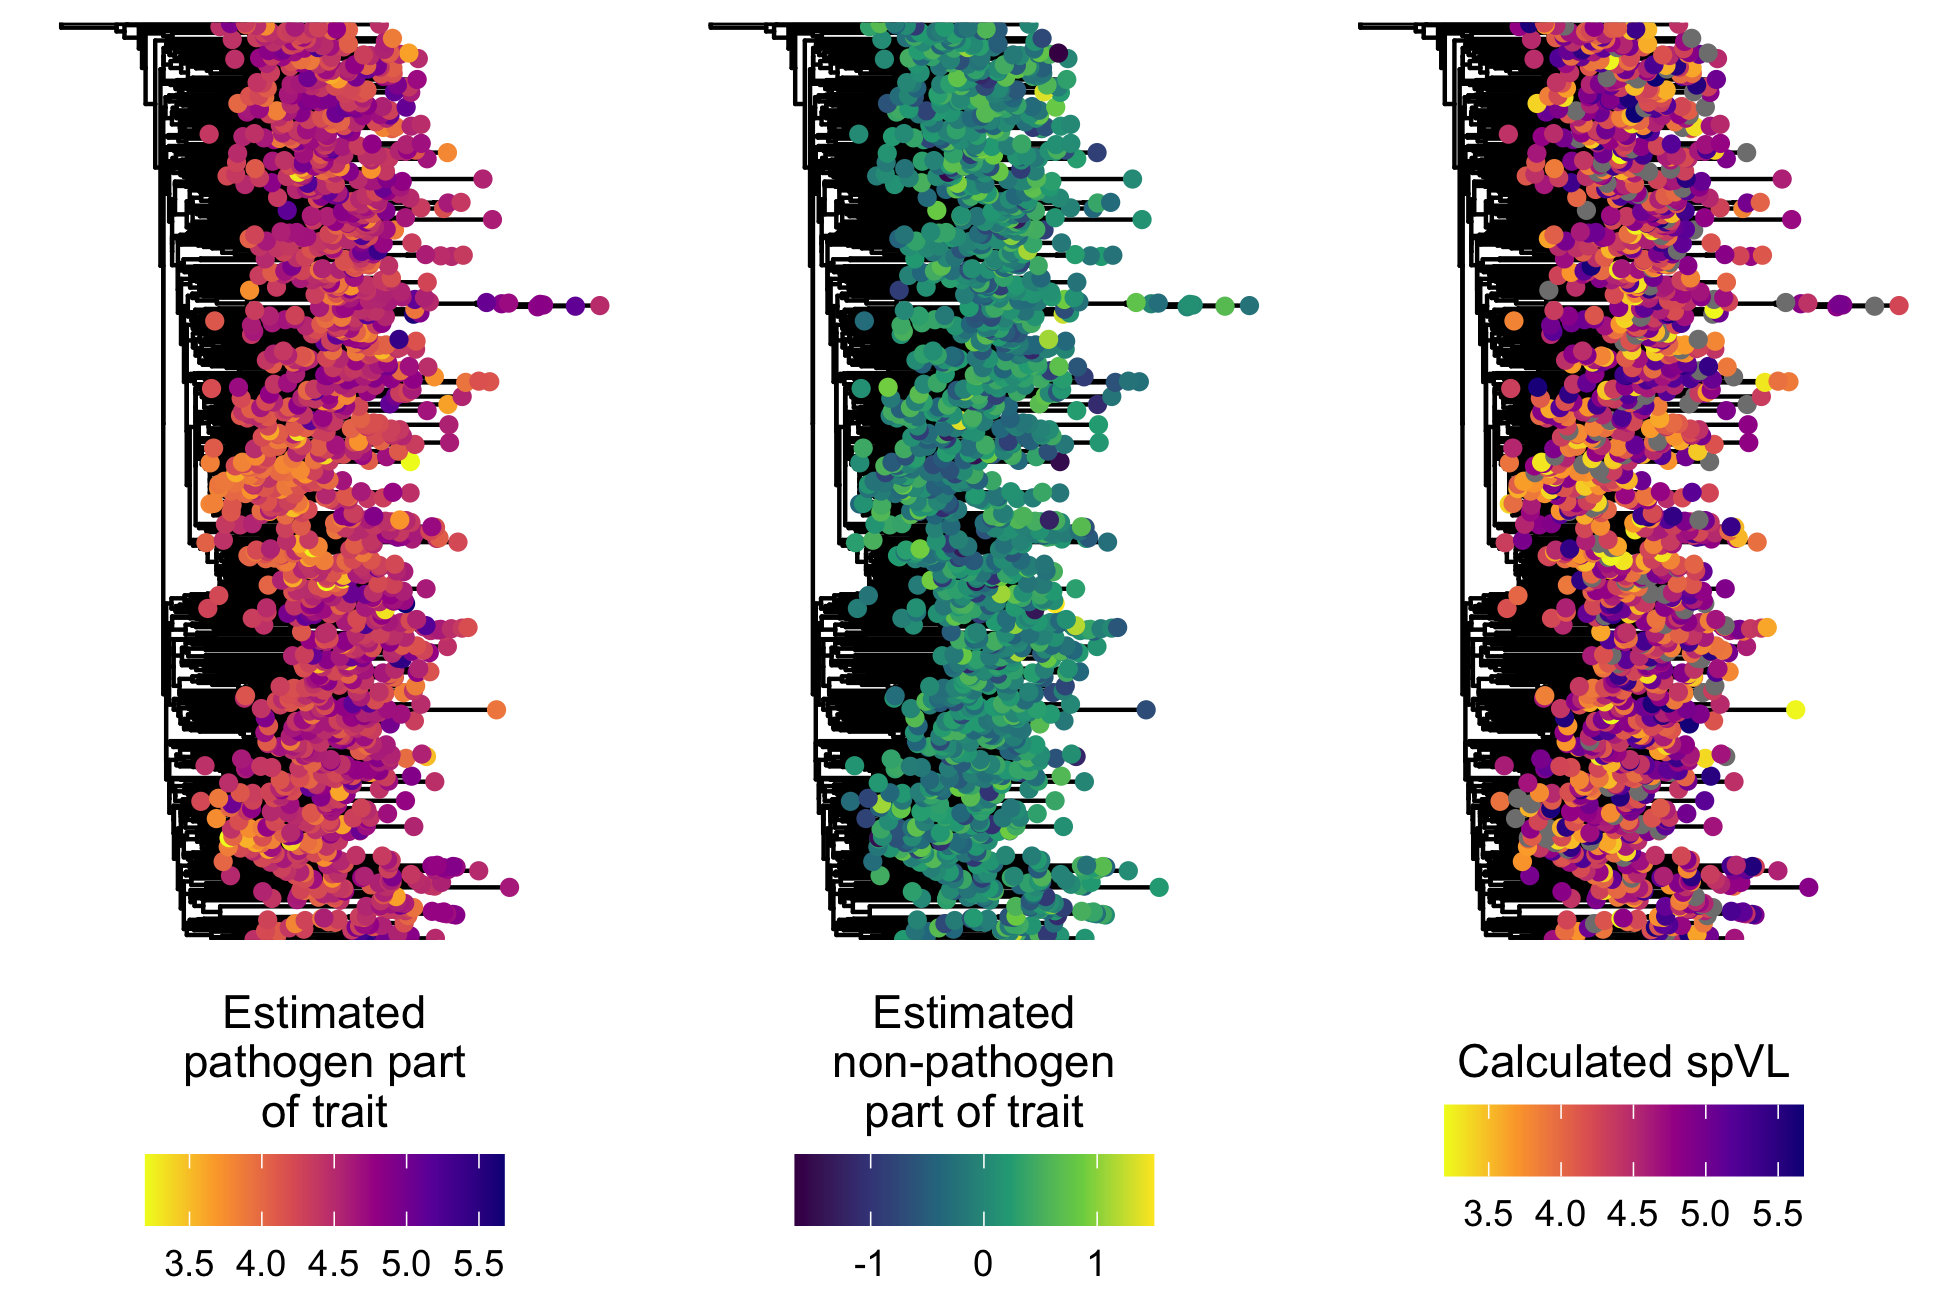
\includegraphics[width = \linewidth]{figures/spvl_on_tree.png}
	\caption{Inferred HIV-1 $pol$ gene phylogeny with tips colored by (A) calculated spVL, (B) estimated non-pathogen effects on spVL and (C) estimated pathogen effects on spVL.}
	\label{fig:spvl-on-tree}
	\end{center}
\end{figure}

\begin{figure}[H]
	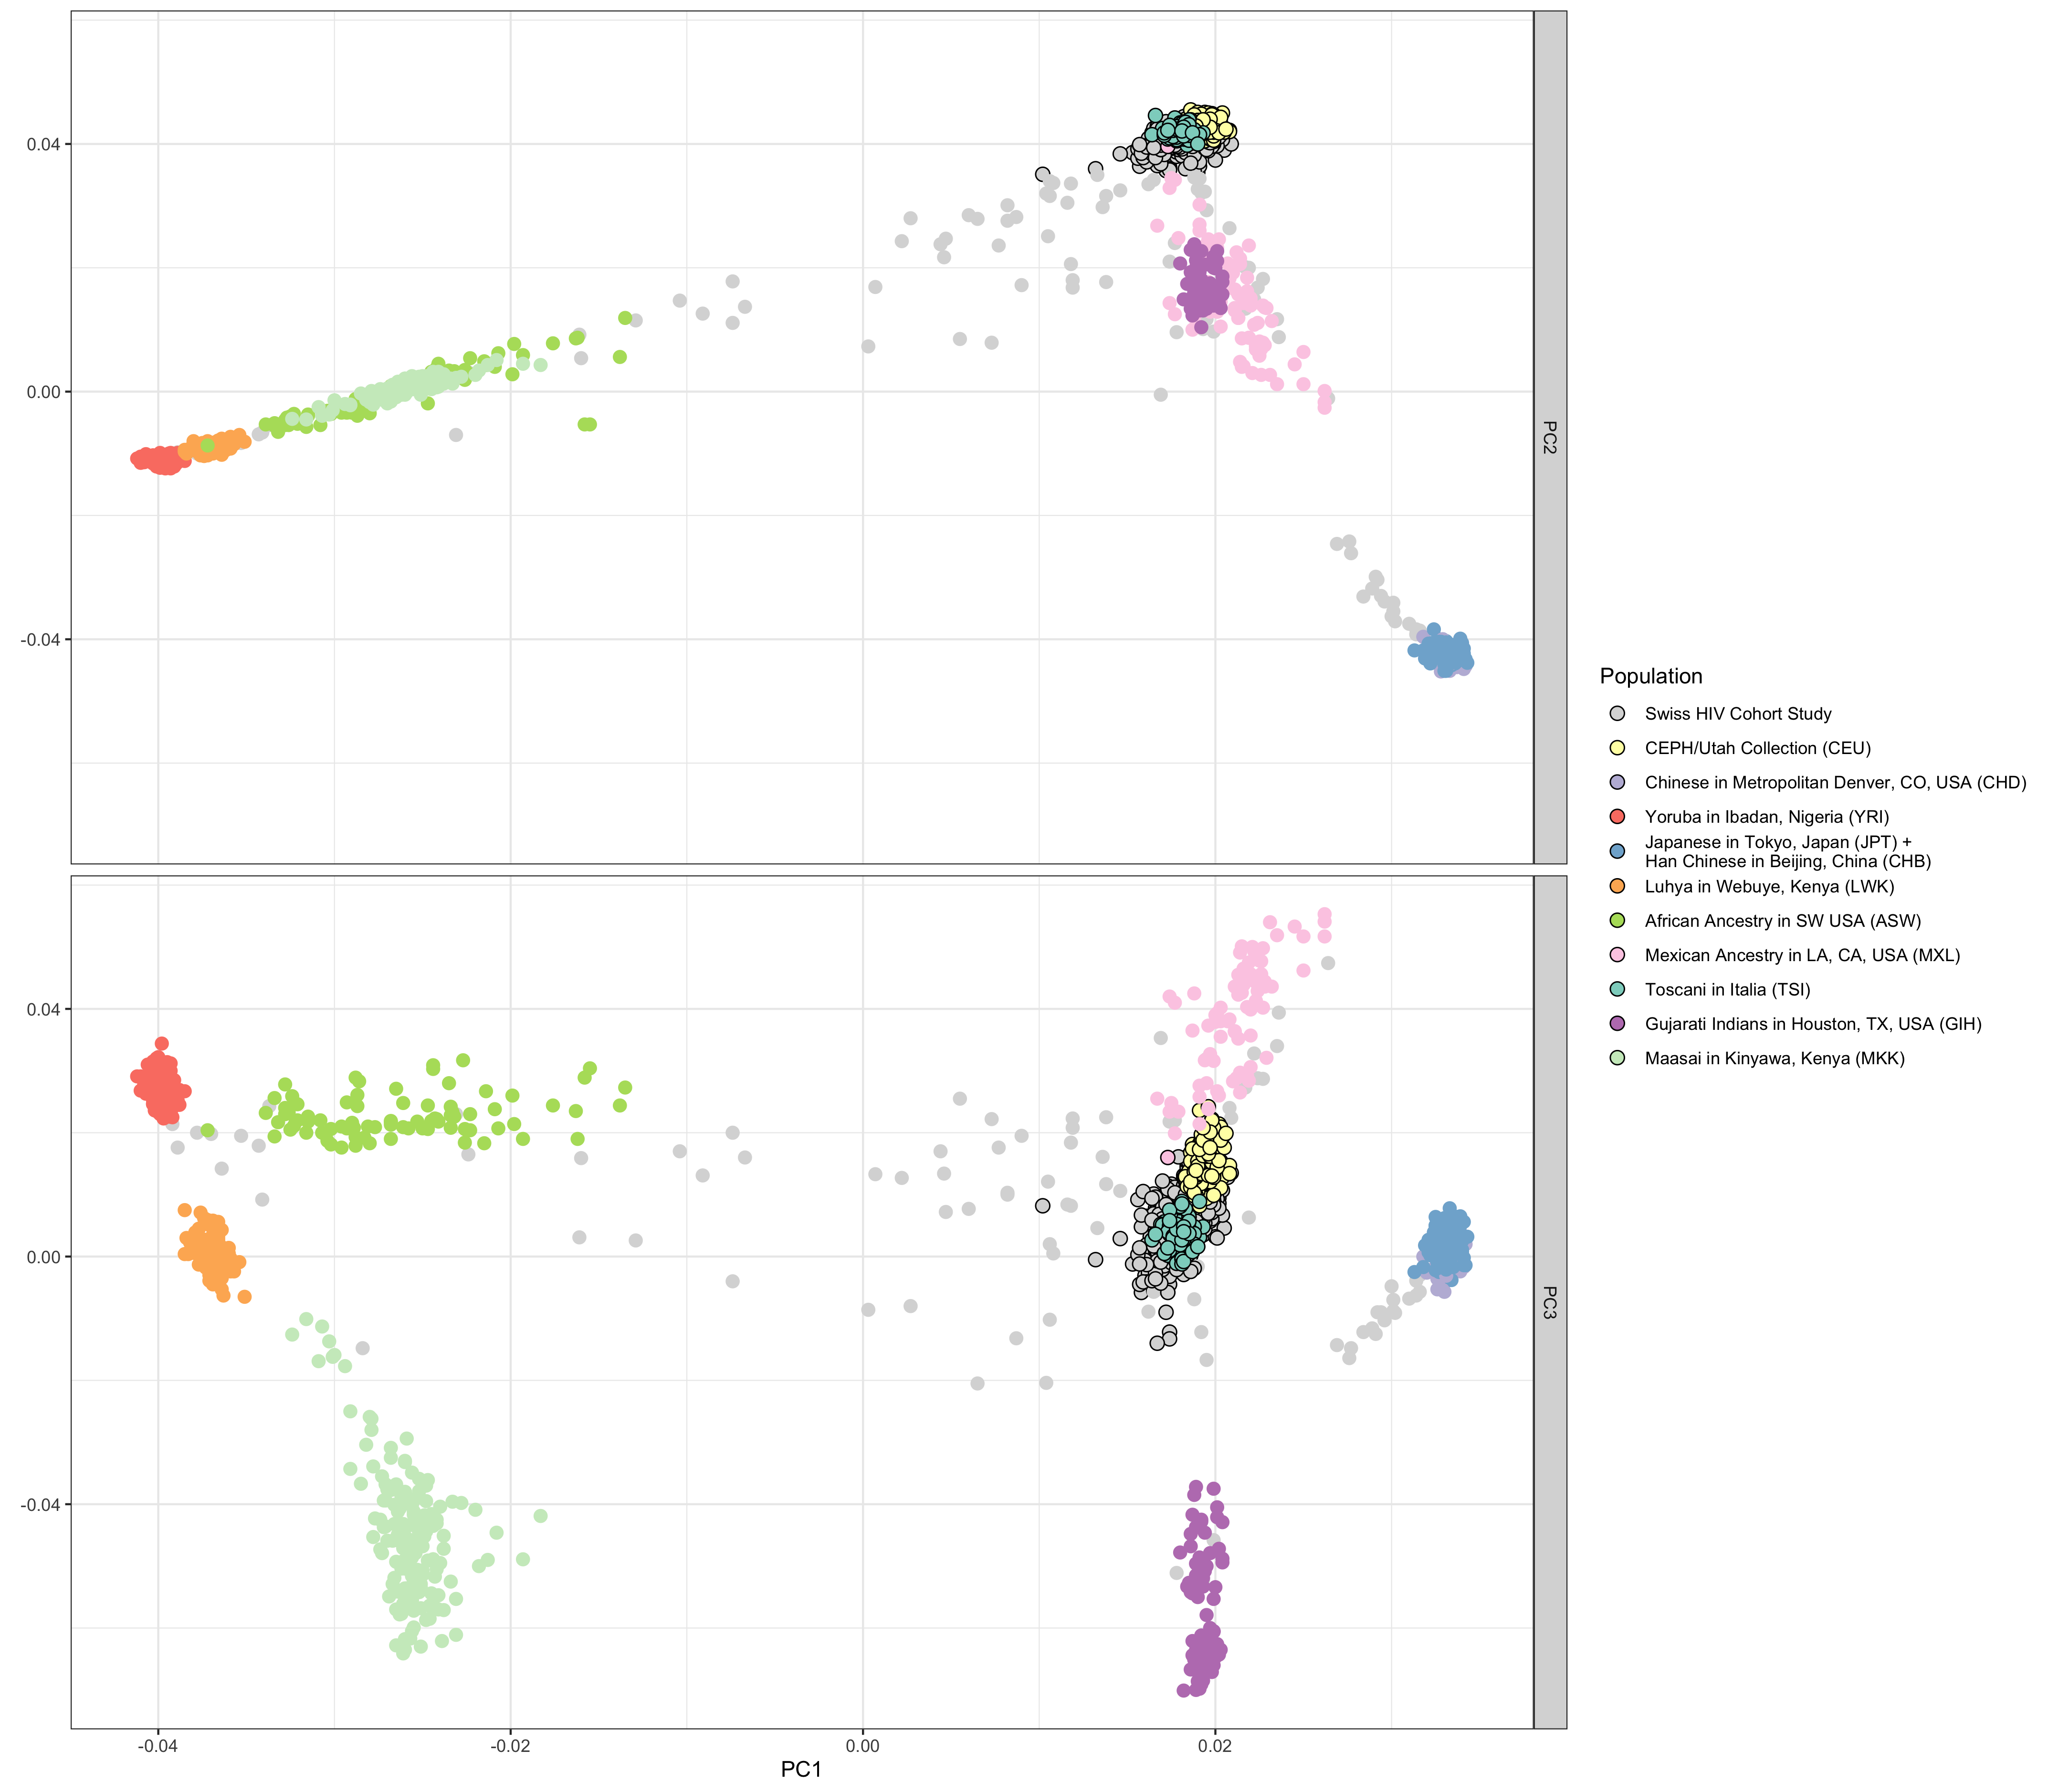
\includegraphics[width=\linewidth]{figures/host_genotype_pca.png}
	\caption{SHCS individuals and HapMap3 individuals plotted along the top three principle components of genetic variation. Points with black borders are within the thresholds used to select individuals of likely European ancestry.}
	\label{fig:PCA}
\end{figure}

\begin{figure}[H]
	\centering
	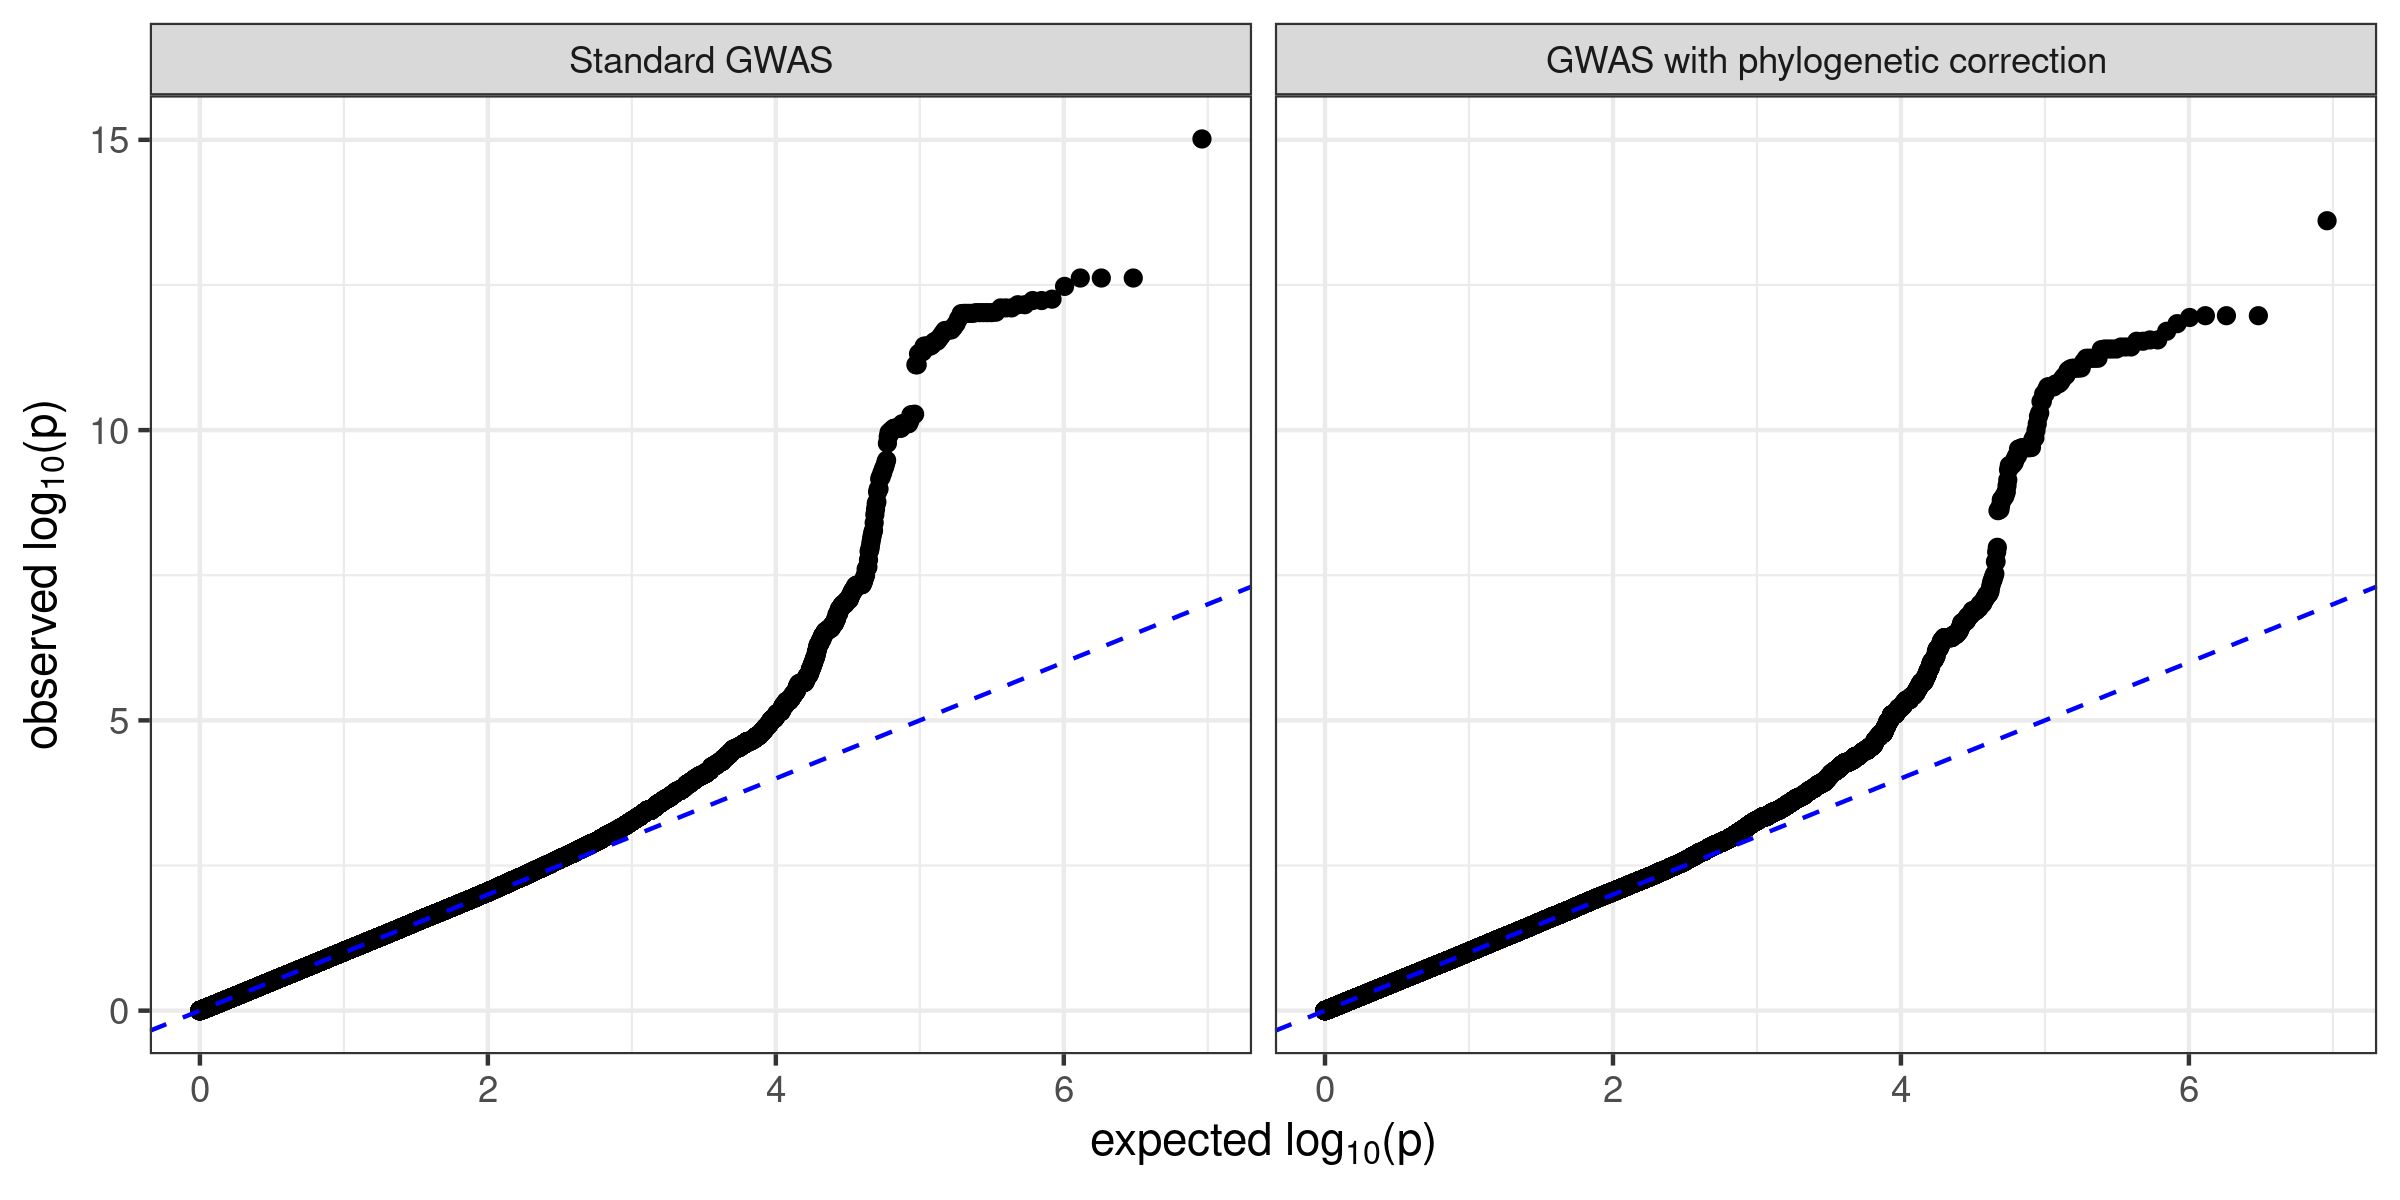
\includegraphics[width=\linewidth]{figures_archived/200207_qq_plots.png}
	\caption{Quartile-quartile plots from association tests.}
	\label{fig:qq-plots}
\end{figure}

\end{doublespace}  % don't doublspace tables

\newpage

\begin{table}[H]
\caption{POUMM parameter estimates for spVL based on Swiss data. HPD = Highest posterior density.}
	\begin{tabular}{lccc} \hline 
	Parameter & Posterior mean & 95\% HPD \\ \hline 
	${g_{0}}$ & 4.23 & (1.72, 6.71) \\
	$\theta$ & 4.47 & (4.37, 4.58) \\
	$\sigma$ & 5.25 & (2.37, 7.9) \\
	$\alpha$ & 57.65 & (19.49, 95.2) \\
	$\sigma_e$ & 0.54 & (0.43, 0.65) \\ 
	$H^2_{\bar{t}}$ & 0.45 & (0.24, 0.67) \\ \hline
	\end{tabular}
	\label{tab:POUMM-parameters}
\end{table}

\begin{table}[H]
\caption{POUMM parameter estimates for spVL from previous studies.}
	\begin{tabular}{lcccp{0.35\linewidth}}
	\hline 
	Parameter & Value & Uncertainty & Reference & Notes \\
	\hline 
	$v_0$ & 5.54 & (4.04 - 7.25) HPD & \citealt{Mitov2018} & 8,483 UK HIV cohort individuals, $pol$ tree \\
	$\theta$ & 4.45 & (4.41 - 4.49) HPD & \citealt{Mitov2018} & \\
	$\theta$ &  4.0 & (1.6 - 4.3) 95\% CI & \citealt{Bertels2018} & 3,036 SHCS individuals, $pol$ tree \\
	$\theta$ & 4.1 & (3.5 - 4.9) 95\% CI & \citealt{Blanquart2017} & 1,581 subtype B individuals from Europe, whole genome tree \\
	$\alpha$ & 28.78 & (16.64 - 46.93) HPD & \citealt{Mitov2018} & \\
	$\alpha$ & 32.7 & (0.03 - 57.6) 95\% CI & \citealt{Bertels2018} & \\
	$\alpha$ & 7.6 & (1.2 - 10) 95\% CI & \citealt{Blanquart2017} & **limited $\alpha$ to $\le$ 10 \\
	$\sigma$ & 2.97 & (1.95 - 4.37) HPD & \citealt{Mitov2018} & \\
	$\sigma$ & 1.3 & (0.66 -1.87) 95\% CI &  \citealt{Blanquart2017} & \\
	$\sigma_e$ & 0.77 & (0.73, 0.8) HPD & \citealt{Mitov2018} & \\
	$\sigma_e$ & 0.61 & (0.54, 0.65) 95\% CI &  \citealt{Blanquart2017} & \\
	\hline 
	\end{tabular}
	\label{tab:POUMMparams}
\end{table}

\begin{table}[H]
\caption{Summary statistics for log spVL in previously sampled populations. $\bar{z}$ is average spVL (log copies/mL) and $\sigma^2_z$ is variance in measured spVL ( log $\textrm{copies}^2/\textrm{mL}^2$). Values from \protect\citet{Blanquart2017, Mitov2018} are empirical; values from \protect\cite{Bonhoeffer2015} were estimated by fitting a normal distribution to the data.}
	\begin{tabular}{lcc} \hline 
	Measurement & Value & Reference \\ \hline 
	$\bar{z}$ & $\approx$ 4.5 & \citealt{Mitov2018} \\
	$\bar{z}$ &  4.4 & \citealt{Blanquart2017} \\
	$\bar{z}$ & $\approx$ 4.5 & \citealt{Bonhoeffer2015} \\
	$\sigma^2_z$ &  0.73 &  \citealt{Mitov2018} \\
	$\sigma^2_z$ &  0.50 & \citealt{Blanquart2017} \\
	$\sigma^2_z$ & $\approx$ 0.5 & \citealt{Bonhoeffer2015} \\ \hline 
	\end{tabular}
	\label{tab:spVLmeasurements}
\end{table}
%\todo{I guessed at bar(z) from figure in Mitov2018, search supplement for exact}

\begin{table}[H]
\caption{Number of samples for GWAS after sequential filtering steps.}
    \begin{tabular}{lc}
    \hline
    Sample filter & Number of samples remaining \\
    \hline
    Subtype B pol sequences & 1516 \\
    With paired spVL measurement & 1516 \\
    $>$ 750 characters in sequence & 1493 \\
    Individual is of European ancestry & 1396 \\
    Kinship coefficient $>$ 0.09375 & 1392 \\ 
    \hline
    \end{tabular}
    \label{tab:sample-filtering}
\end{table}

\begin{table}[H]
\caption{Number of variants for GWAS after sequential filtering steps.}
	\begin{tabular}{lc}
	\hline
	Variant filter & Number of variants remaining \\
	\hline 
	Raw data & 76979521 \\
	Missing genotype rate $>$ 0.01 & 7452957 \\
	Hardy-Weinburg exact test p-value $<$ 5x10$^-5$ & 7452425 \\
	Minor allele frequency $<$ 0.01 & 4556770 \\ \hline			
	\end{tabular}
	\label{tab:variant-filtering}
\end{table}

\begin{longtable}[H]{lp{1cm}p{2cm}p{1cm}p{2cm}p{1cm}p{2cm}} % {lrrrrrr}{lrrrrrr}
		\caption{Association results for common class I HLA alleles ranked by p-value from the GWAS by \citet{McLaren2015} compared to results from the current study.}
		\hline
		& \multicolumn{2}{l}{McLaren et al.}  & \multicolumn{2}{l}{Standard GWAS} & \multicolumn{2}{l}{GWAS with phylogenetic correction} \\ 
		\hline
	 	Allele & Beta & p-value & Beta &p-value & Beta& p-value \\ 
		\hline
		HLA-B*57:01 & -0.840 & $2.69 \times 10^{-86}$ & -0.479 & $1.11 \times 10^{-12}$ & -0.268 & $5.43 \times 10^{-12}$ \\ 
		HLA-C*06:02 & -0.436 & $7.32 \times 10^{-50}$ & -0.173 & $1.10 \times 10^{-4}$ & -0.107 & $3.15 \times 10^{-5}$ \\ 
		HLA-B*27:05 & -0.417 & $4.32 \times 10^{-20}$ & -0.244 & $9.59 \times 10^{-4}$ & -0.122 & $4.40 \times 10^{-3}$ \\ 
		HLA-C*07:01 & 0.195 & $1.86 \times 10^{-14}$ & 0.129 & $7.55 \times 10^{-3}$ & 0.086 & $1.99 \times 10^{-3}$ \\ 
		HLA-C*07:02 & 0.194 & $3.75 \times 10^{-13}$ & 0.095 & $3.02 \times 10^{-2}$ & 0.052 & $3.98 \times 10^{-2}$ \\ 
		HLA-B*07:02 & 0.200 & $5.17 \times 10^{-13}$ & 0.129 & $5.29 \times 10^{-3}$ & 0.072 & $7.06 \times 10^{-3}$ \\ 
		HLA-B*08:01 & 0.206 & $2.94 \times 10^{-11}$ & -0.009 & $9.20 \times 10^{-1}$ & 0.015 & $7.75 \times 10^{-1}$ \\ 
		HLA-C*08:02 & -0.307 & $8.76 \times 10^{-11}$ & 0.324 & $8.55 \times 10^{-1}$ & 0.400 & $6.95 \times 10^{-1}$ \\ 
		HLA-C*04:01 & 0.183 & $9.07 \times 10^{-11}$ & 0.124 & $3.04 \times 10^{-3}$ & 0.058 & $1.67 \times 10^{-2}$ \\ 
		HLA-B*13:02 & -0.346 & $3.70 \times 10^{-10}$ & -0.188 & $1.03 \times 10^{-2}$ & -0.112 & $7.90 \times 10^{-3}$ \\ 
		HLA-B*14:02 & -0.318 & $2.10 \times 10^{-9}$ & 0.067 & $8.12 \times 10^{-1}$ & 0.118 & $4.71 \times 10^{-1}$ \\ 
		HLA-C*12:02 & -0.478 & $4.02 \times 10^{-8}$ & 0.111 & $7.63 \times 10^{-1}$ & 0.094 & $6.58 \times 10^{-1}$ \\ 
		HLA-C*02:02 & -0.223 & $5.45 \times 10^{-8}$ & -0.089 & $1.31 \times 10^{-1}$ & -0.039 & $2.50 \times 10^{-1}$ \\ 
		HLA-A*25:01 & -0.301 & $6.80 \times 10^{-8}$ & -0.090 & $9.93 \times 10^{-2}$ & -0.033 & $2.96 \times 10^{-1}$ \\ 
		HLA-B*52:01 & -0.435 & $2.60 \times 10^{-7}$ & 0.238 & $7.63 \times 10^{-2}$ & 0.150 & $5.33 \times 10^{-2}$ \\ 
		HLA-C*01:02 & -0.231 & $2.22 \times 10^{-6}$ & -0.198 & $5.07 \times 10^{-4}$ & -0.113 & $5.70 \times 10^{-4}$ \\ 
		HLA-A*23:01 & 0.269 & $1.66 \times 10^{-5}$ & 0.020 & $7.42 \times 10^{-1}$ & 0.015 & $6.59 \times 10^{-1}$ \\ 
		HLA-B*55:01 & 0.302 & $2.32 \times 10^{-5}$ & 0.685 & $2.48 \times 10^{-1}$ & 0.436 & $2.03 \times 10^{-1}$ \\ 
		HLA-B*35:02 & 0.358 & $2.42 \times 10^{-5}$ &  &  &  &  \\ 
		HLA-A*31:01 & -0.219 & $4.36 \times 10^{-5}$ & -0.052 & $4.50 \times 10^{-1}$ & -0.017 & $6.78 \times 10^{-1}$ \\ 
		HLA-B*35:01 & 0.156 & $4.82 \times 10^{-5}$ & 0.167 & $2.13 \times 10^{-4}$ & 0.083 & $1.33 \times 10^{-3}$ \\ 
		HLA-B*49:01 & 0.253 & $1.86 \times 10^{-4}$ & 2.173 & $9.79 \times 10^{-4}$ & 1.253 & $9.82 \times 10^{-4}$ \\ 
		HLA-B*35:03 & 0.215 & $7.13 \times 10^{-4}$ & -0.241 & $8.00 \times 10^{-1}$ & 0.261 & $6.35 \times 10^{-1}$ \\ 
		HLA-B*40:01 & 0.148 & $9.37 \times 10^{-4}$ & 0.519 & $1.06 \times 10^{-2}$ & 0.349 & $2.91 \times 10^{-3}$ \\ 
		HLA-B*18:01 & 0.136 & $9.48 \times 10^{-4}$ & 0.208 & $1.73 \times 10^{-3}$ & 0.133 & $5.09 \times 10^{-4}$ \\ 
		HLA-A*29:02 & 0.167 & $1.40 \times 10^{-3}$ & 0.150 & $6.17 \times 10^{-2}$ & 0.092 & $4.72 \times 10^{-2}$ \\ 
		HLA-C*14:02 & -0.228 & $1.50 \times 10^{-3}$ & 0.266 & $7.59 \times 10^{-1}$ & 0.235 & $6.38 \times 10^{-1}$ \\ 
		HLA-A*11:01 & -0.109 & $2.70 \times 10^{-3}$ & -0.090 & $8.96 \times 10^{-2}$ & -0.052 & $8.92 \times 10^{-2}$ \\ 
		HLA-A*24:02 & 0.094 & $3.60 \times 10^{-3}$ & 0.133 & $3.79 \times 10^{-3}$ & 0.074 & $5.52 \times 10^{-3}$ \\ 
		HLA-B*37:01 & 0.222 & $4.50 \times 10^{-3}$ & 0.600 & $3.22 \times 10^{-3}$ & 0.311 & $8.11 \times 10^{-3}$ \\ 
		HLA-B*44:03 & 0.119 & $5.00 \times 10^{-3}$ & -0.114 & $2.77 \times 10^{-1}$ & -0.080 & $1.88 \times 10^{-1}$ \\ 
		HLA-C*03:03 & 0.110 & $6.50 \times 10^{-3}$ & -0.078 & $1.86 \times 10^{-1}$ & -0.031 & $3.66 \times 10^{-1}$ \\ 
		HLA-B*58:01 & -0.253 & $7.10 \times 10^{-3}$ & 6.895 & $7.93 \times 10^{-2}$ & 4.841 & $3.27 \times 10^{-2}$ \\ 
		HLA-A*32:01 & -0.123 & $8.30 \times 10^{-3}$ & 0.089 & $5.31 \times 10^{-1}$ & 0.071 & $3.86 \times 10^{-1}$ \\ 
		HLA-C*16:01 & 0.137 & $8.60 \times 10^{-3}$ & 0.057 & $4.46 \times 10^{-1}$ & 0.013 & $7.60 \times 10^{-1}$ \\ 
		HLA-C*03:04 & 0.093 & $1.25 \times 10^{-2}$ & 0.126 & $3.52 \times 10^{-2}$ & 0.095 & $5.77 \times 10^{-3}$ \\ 
		HLA-B*38:01 & -0.148 & $1.35 \times 10^{-2}$ & -3.459 & $3.01 \times 10^{-1}$ & -2.224 & $2.49 \times 10^{-1}$ \\ 
		HLA-A*33:01 & -0.233 & $1.45 \times 10^{-2}$ &  &  &  &  \\ 
		HLA-A*30:01 & -0.159 & $2.89 \times 10^{-2}$ & 0.072 & $9.04 \times 10^{-1}$ & 0.008 & $9.82 \times 10^{-1}$ \\ 
		HLA-C*12:03 & -0.077 & $4.59 \times 10^{-2}$ & -0.114 & $2.95 \times 10^{-2}$ & -0.067 & $2.68 \times 10^{-2}$ \\ 
		HLA-A*01:01 & 0.051 & $4.78 \times 10^{-2}$ & -0.039 & $4.88 \times 10^{-1}$ & -0.050 & $1.24 \times 10^{-1}$ \\ 
		HLA-B*14:01 & -0.187 & $5.51 \times 10^{-2}$ & 7.071 & $5.00 \times 10^{-2}$ & 3.974 & $5.62 \times 10^{-2}$ \\ 
		HLA-B*40:02 & -0.130 & $1.01 \times 10^{-1}$ & -0.343 & $3.88 \times 10^{-1}$ & -0.105 & $6.47 \times 10^{-1}$ \\ 
		HLA-C*07:04 & 0.125 & $1.02 \times 10^{-1}$ & 0.111 & $3.00 \times 10^{-1}$ & 0.080 & $1.98 \times 10^{-1}$ \\ 
		HLA-C*05:01 & 0.043 & $1.93 \times 10^{-1}$ & -0.022 & $6.51 \times 10^{-1}$ & -0.019 & $4.82 \times 10^{-1}$ \\ 
		HLA-A*03:01 & 0.025 & $3.29 \times 10^{-1}$ & 0.002 & $9.51 \times 10^{-1}$ & -0.001 & $9.81 \times 10^{-1}$ \\ 
		HLA-B*51:01 & -0.036 & $3.52 \times 10^{-1}$ & -0.046 & $3.13 \times 10^{-1}$ & -0.044 & $1.01 \times 10^{-1}$ \\ 
		HLA-A*68:01 & 0.046 & $3.71 \times 10^{-1}$ & 0.036 & $6.09 \times 10^{-1}$ & 0.009 & $8.27 \times 10^{-1}$ \\ 
		HLA-B*44:02 & 0.030 & $3.73 \times 10^{-1}$ & -0.051 & $3.90 \times 10^{-1}$ & -0.031 & $3.57 \times 10^{-1}$ \\ 
		HLA-B*39:01 & 0.073 & $3.85 \times 10^{-1}$ &  &  &  &  \\ 
		HLA-A*02:01 & 0.017 & $3.94 \times 10^{-1}$ & -0.018 & $5.57 \times 10^{-1}$ & -0.008 & $6.77 \times 10^{-1}$ \\ 
		HLA-C*15:02 & -0.046 & $4.20 \times 10^{-1}$ & 0.064 & $3.26 \times 10^{-1}$ & 0.033 & $3.78 \times 10^{-1}$ \\ 
		HLA-B*50:01 & 0.066 & $4.68 \times 10^{-1}$ & 1.522 & $1.77 \times 10^{-2}$ & 0.970 & $8.73 \times 10^{-3}$ \\ 
		HLA-B*15:01 & -0.021 & $5.71 \times 10^{-1}$ & -0.073 & $1.71 \times 10^{-1}$ & -0.021 & $4.93 \times 10^{-1}$ \\ 
		HLA-A*30:02 & 0.050 & $5.92 \times 10^{-1}$ & 0.047 & $9.28 \times 10^{-1}$ & -0.004 & $9.89 \times 10^{-1}$ \\ 
		HLA-A*26:01 & -0.003 & $9.57 \times 10^{-1}$ & -0.645 & $1.96 \times 10^{-1}$ & -0.529 & $6.59 \times 10^{-2}$ \\
		\hline
		\label{tab:full-mclaren-comparison}
\end{longtable}

% \begin{figure}[H]
% 	\includegraphics[width=\linewidth]{images/HIV_tree_branch_lengths}
% 	\caption{Left plot: branch length distributions for UK HIV tree and our simulated HIV tree prior to pruning down to 500 tips. The mean root-to-tip distance for the UK tree is 0.14 and the mean branch length is 0.02. The mean root-to-tip distance for the full simulated HIV tree is 0.14 and the mean branch length is 0.01. Right plot: branch length distribution for the tree of 500 tips used for simulation. The mean root-to-tip distance for the pruned HIV tree is 0.14 and the mean branch length is 0.03.}
% 	\label{fig:branchlengths}
% \end{figure}

\typeout{}
\printbibliography

\end{document}

%\citet{Mitov2018} and \citet{Bertels2018} both found higher statistical support for the POUMM model of spVL evolution as opposed to the corresponding model assuming Brownian motion only. This makes sense in the context of the hypothesis proposed by \citet{Fraser2014}, in which spVL is under stabilizing selection to maximize transmissibility of the virus. On the other hand, the assumptions that $e$ are normally distributed, mutually indpendent, and have an expected value of 0 are consistent with the idea that genetic effects from several unlinked host loci and environmental effects from many independent factors are each equally likely to increase an individual's spVL as decrease it. \todo{This statement is not supported}
%
%\todo{TBD once we have real data, here are some thoughts}
%The success of our method in identifying new host determinants of spVL depends on how much host-determined variation in spVL actually exists. In the largest GWAS for HIV spVL to date, \citet{McLaren2015} estimated that additive effects from common human genetic variants explain 20\% of the variability in spVL. Of this quantity, 94.5\% was attributable to variants in just two regions in the human genome. \todo{Were there variants other than HLA in the MHC region?} Associations were with alleles in the CCR5 gene, which encodes a co-receptor for HIV entry into CD4+ T-cells, and the human leukocyte antigen (HLA) genes, which encode proteins that present certain host and pathogen-derived peptides at the surface of cells. These associations have been well-replicated in several GWAS \citet{Naranbhai2017}. This results suggest that nearly all host-determined variation in spVL can be explained by previously discovered variants. 
%
%In a joint analysis of both host and viral genotypes, \citet{Bartha2017} showed that nearly all of the variation in spVL explained by human genetic variation overlaps that explained by HIV genetic variation. If this is the case then our method to remove the viral contribution to spVL prior to GWAS should yield only associations between host variants and spVL that are independent of the virus. Additionally, effect size estimates for associations will reflect only the effect of the host variant, not any correlated effect from the virus.

%\subsection{New method to estimate the viral and non-viral parts of spVL}
%
%Here we derive a method to estimate the viral part of spVL for each infected host by assuming that spVL values at the tips of a phylogenetic tree $\mathcal{T}$ have evolved under the POUMM. In particular, for every tip $i$ in the tree, we assume that the host’s spVL value, $z_i$, is formed as a sum of three independent parts: a  heritable part determined by additive genetic effects from the virus, $g_{v_i}$, a non-heritable part determined by additive genetic effects from the host, $g_{h_i}$, and a further non-heritable part, $\epsilon_i$, which encompasses any other factor effecting spVL (Equation \ref{eq:totalspVL}). For the purposes of our derivation, it is convent to combine the non-heritable parts of spVL, $g_{h_i} + \epsilon_i$, into a single variable $e_i$.
%
%\begin{align} 
%z _i &= g_{v_i} + g_{h_i} + \epsilon_i \\
%\xrightarrow{e_i = g_{h_i} + \epsilon_i } z_i &= g_{v_i} + e_i  \label{eq:totalspVL}
%\end{align}
%
%According to the POUMM, the unobserved viral component of spVL for each host, $g_{v_i}$, evolves along the tree according to an Ornstein-Uhlenbeck (OU) process. The OU process was first introduced by \citet{Lande1976} as a model of evolution under both drift and stabilizing selection, so we are assuming $g_{v_i}$ continually evolves towards an evolutionary optimum in each viral lineage but is subject to random evolutionary fluctuations. Mathematically, $g_{v_i}$ is a realization of a Gaussian distributed random variable $G_{v_i} \sim \mathcal{N}(\mu_{OU_i}, \sigma^2_{OU_i})$, where:
%
%\begin{equation} \label{eq:muOU}
%\mu_{OU_i} = z_0e^{-\alpha t_{0i}} + (1 - e^{-\alpha t_{0i}})\theta \\
%\end{equation}
%\begin{equation}\label{eq:sigOU}
%	\sigma^2_{OU_i} = \sigma^2\frac{(1 - e^{-2\alpha t_{0i}})}{2\alpha}
%\end{equation}
%
%$z_0$ is the ancestral spVL value at the root of the tree, $\theta$ is the optimal spVL value that maximizes viral fitness,  $\alpha$ is the strength of selection on spVL, and $\sigma$ is the standard deviation of random fluctuations in $g_{v}$. We refer to these OU parameters ($z_0, \theta, \alpha, \textrm{and } \sigma$) collectively as $\Theta$. Finally, $t_{0i}$ is the phylogenetic distance from the root of the tree to tip $i$. We use the following notation to denote that the distribution of $G_{v}$ depends on the tree, $\mathcal{T}$, and the OU parameters $\Theta$: $G_{v|\Theta, \mathcal{T}}$. Generalizing to $N$ total tips in the tree, $\vec{G}_{v|\Theta, \mathcal{T}} = (G_{v_1}, ..., G_{v_N})^T$ is a random vector for the unobserved viral component of spVL at the tips. We know that $\vec{G}_{v|\Theta, \mathcal{T}} \sim \mathcal{N}(\vec{\mu}_{OU}, \mathbf{\Sigma}_{OU})$, where the elements of the variance-covariance matrix $\mathbf{\Sigma}_{OU}$ are calculated as follows:
%
%\begin{align} 
%\bm{\Sigma}_{OU_{ii}} &= \sigma^2\frac{(1 - e^{-2\alpha t_{0i}})}{2\alpha} \label{eq:SigmaOUii} \\
%\bm{\Sigma}_{OU_{ij}}&= \sigma^2\frac{e^{-\alpha\tau_{ij}}(1 - e^{-2\alpha t_{0(ij)}})}{2\alpha} \label{eq:SigmaOUij}
%\end{align}
%
%$\tau_{ij}$ is the phylogenetic distance between tips $i$ and $j$ and $t_{0(ij)}$ is the phylogenetic distance from the root of the tree to the most recent common ancestor of $i$ and $j$. Equations \ref{eq:muOU}, \ref{eq:SigmaOUii}, and \ref{eq:SigmaOUij} completely describe the generating process for the unobserved viral part of spVL under the assumptions of the POUMM. 
%
%On the other hand, the non-heritable component of spVL for each host, $e_i$ is assumed to be normally distributed in the population with an expected value of zero.  Furthermore, $e_i$ is uncorrelated among hosts and independent of the heritable viral part of spVL. Mathematically, $e_i$, is a realization of another Gaussian distributed random variable $E_i \sim \mathcal{N}(0, \sigma^2_e)$, which is independent of $G_{v_j}$ for any tip $j$. $\vec{E}_{|\sigma_e} = (E_1, ..., E_N)^T$ is a random vector for the unobserved non-viral part of spVL at the tips. The parameter $\sigma_e$ is the standard deviation of the non-viral component of spVL in the population. 
% 
% \begin{theorem}\label{thmGValues}
% 	Given the POUMM assumptions described, the pair of random vectors $<\vec{G}_{|\Theta,\mathcal{T},\sigma_e, \vec{z}},\vec{E}_{|\Theta,\mathcal{T}, \sigma_e, \vec{z}} >$ satisfies the following:
% 	\begin{enumerate}
% 		\renewcommand{\theenumi}{\alph{enumi}}
% 		\item Each realisation $\vec{g_v}_{|\Theta,\mathcal{T}, \sigma_e, \vec{z}}$ of $\vec{G_v}_{|\Theta,\mathcal{T},\sigma_e, \vec{z}}$ is also a realization of $\vec{G}_{|\Theta, \mathcal{T}}$, i.e. it results from simulating the OU branching process defined by $\Theta$ on $\mathcal{T}$;
% 		\item $\vec{E}_{|\Theta,\mathcal{T}, \sigma_e, \vec{z}} = \vec{z} - \vec{G_v}_{|\Theta,\mathcal{T}, \sigma_e, \vec{z}}$, i.e. each realization $\vec{e}_{|\Theta,\mathcal{T}, \sigma_e, \vec{z}}$ of $\vec{E}_{|\Theta,\mathcal{T}, \sigma_e, \vec{z}}$  satisfies $\vec{z} = \vec{g}_{|\Theta,\mathcal{T}, \sigma_e, \vec{z}} + \vec{e}_{|\Theta,\mathcal{T}, \sigma_e, \vec{z}}$ for its corresponding realization $\vec{g}_{|\Theta,\mathcal{T}, \sigma_e, \vec{z}}$  of $\vec{G}_{|\Theta,\mathcal{T}, \sigma_e, \vec{z}}$ in the same pair.
% 	\end{enumerate}
% 	Then the pdf of $<\vec{G}_{|\Theta,\mathcal{T},\sigma_e, \vec{z}},\vec{E}_{|\Theta,\mathcal{T}, \sigma_e, \vec{z}} >$ is proportional to a $N$-variate Gaussian function, i.e. 
% 	\begin{equation}\label{eqPdfGValues1}
% 	f\big(<\vec{g}_{|\\Theta,\mathcal{T},\sigma_e, \vec{z}}, \vec{e}_{|\Theta,\mathcal{T}, \sigma_e, \vec{z}}>\big) \propto \mathcal{N}\big(\vec{g}_{|\Theta,\mathcal{T}, \sigma_e, \vec{z}}\ ;\ \vec{\mu}_{MWA}(\Theta,\mathcal{T}, \sigma_e, \vec{z}), \mathbf{\Sigma}_{MWA}(\Theta,\mathcal{T}, \sigma_e, \vec{z})\big),
% 	\end{equation}
% 	\noindent where the matrix $\mathbf{\Sigma}_{MWA}(\Theta,\mathcal{T}, \sigma_e, \vec{z})$ and the  vector $\vec{\mu}_{MWA}(\Theta,\mathcal{T}, \sigma_e, \vec{z})$ are defined as follows:
% 	\begin{equation}\label{eqMuSigmaGValues}
% 	\begin{array}{rcl}
% 	\mathbf{\Sigma}_{MWA}(\Theta,\mathcal{T},\sigma_e) & = & \bigg(\big[\mathbf{\Sigma}_{OU}(\Theta,\mathcal{T})\big]^{-1}+\mathbf{\Sigma}_{e}(\sigma_e)^{-1}\bigg)^{-1}\\
% 	\vec{\mu}_{MWA}(\Theta,\mathcal{T},\sigma_e, \vec{z}) & = & \mathbf{\Sigma}_{MWA}(\Theta,\mathcal{T},\sigma_e) \bigg(\big[\mathbf{\Sigma}_{OU}(\Theta,\mathcal{T})\big]^{-1}\vec{\mu}_{OU}(\Theta,\mathcal{T}) +  \mathbf{\Sigma}_{e}(\sigma_e)^{-1} \vec{z}\bigg).
% 	\end{array}
% 	\end{equation}
% \end{theorem}
% \begin{proof}
% 	\begin{equation}\label{eqPdfGValues2}
% 	\begin{array}{rcl}
% 	f\big(<\vec{g}_{|\Theta,\mathcal{T},\sigma_e,\vec{z}},\ \vec{e}_{|\Theta,\mathcal{T},\sigma_e,\vec{z}}>\big) & = & f\big(\vec{g}_{|\Theta,\mathcal{T},\sigma_e,\vec{z}}\ |\ \vec{e}_{|\Theta,\mathcal{T},\sigma_e,\vec{z}}\big) \times f\big(\vec{e}_{|\Theta,\mathcal{T},\sigma_e,\vec{z}}\big)\\
% 	& = &\mathcal{N}\bigg(\vec{g}_{|\Theta,\mathcal{T},\sigma_e,\vec{z}}\ ;\ \vec{\mu}_{OU}(\Theta,\mathcal{T}), \mathbf{\Sigma}_{OU}(\Theta,\mathcal{T})\bigg) \times \\
% 	& &  \mathcal{N}\bigg(\vec{z} - \vec{g}_{|\Theta,\mathcal{T},\sigma_e,\vec{z}}\ ;\ \vec{0}, \mathbf{\Sigma}_e(\sigma_e)\bigg) \\
% 	& = & \mathcal{N}\bigg(\vec{g}_{|\Theta,\mathcal{T},\sigma_e,\vec{z}}\ ;\ \vec{\mu}_{OU}(\Theta,\mathcal{T}), \mathbf{\Sigma}_{OU}(\Theta,\mathcal{T})\bigg) \times \\
% 	& &  \mathcal{N}\bigg(\vec{g}_{|\Theta,\mathcal{T},\sigma_e,\vec{z}}\ ;\  \vec{z}, \mathbf{\Sigma}_e(\sigma_e)\bigg) \\
% 	\end{array}
% 	\end{equation}
% 	
% 	Equations \ref{eqPdfGValues1} and \ref{eqMuSigmaGValues} follow from eq. \ref{eqPdfGValues2} and eq. 371, p. 42, section 8.1.8 ``Product of Gaussian densities'' in \citet{Petersen2012}.
% 	
% \end{proof}
%
%Removing the viral part of spVL from total spVL using the above method results in the following ordinary least squares slope and intercept coefficient estimates for GWAS:
%
%\begin{equation} \label{eq: OLS-soln}
%	\hat{\beta}_i = (\mathbf{X}_i^T\mathbf{X}_i)^{-1}\mathbf{X}_i^T(\vec{z} - \vec{\mu}_{MWA})
%\end{equation}
%
%where $\mathbf{X}_i$ is the $N \times 2$ design matrix of host genotypes for genetic variant $i$.
%\begin{equation*}
%	\mathbf{X}_i = \begin{bmatrix}
%	1 & g_{i1}  \\
%	\vdots & \vdots \\
%	1 & g_{iN} 
%	\end{bmatrix}
%\end{equation*}
%
%%  serves three purposes. 1) We can estimate for each patient the effect the virus has on their spVL; 2) we can  account for non-independence between spVL samples due to the viral phylogeny; and 3) we can generate corrected estimates for each host genetic variant's effect on spVL, excluding any effect of the virus.
% 
%\subsection{PGLS}
%
%We made two notable changes to the typical PGLS framework (see \citealt{Garamszegi2014} for a nice overview of PGLS). First, we assumed a variance-covariance structure for regression residuals according to the POUMM. This matrix equals $\mathbf{\Sigma}_{OU} + \mathbf{\Sigma}_{e}$. Second, we use the variances on the diagonal of this matrix as sample weights to account for non-ultrametricity of the HIV tree. We implemented PGLS including these two modifications using the nmle package in R \parencite{Pinheiro2019}. The resulting general least squares slope and intercept coefficient estimates for GWAS are:
%
%\begin{equation}
%	\hat{\beta}_i = (\mathbf{X}_i^T(\mathbf{\Sigma}_{OU} + \mathbf{\Sigma}_e)^{-1}\mathbf{X}_i)^{-1}\mathbf{X}_i^T(\mathbf{\Sigma}_{OU} + \mathbf{\Sigma}_e)^{-1}\vec{z}
%\end{equation}
 
% \subsection{Comparison to PGLS}
% 
%We now adopt a second method to correct GWAS for the viral phylogeny by borrowing a method long used by evolutionary biologists. Phylogenetic generalized least squares (PGLS) regression is a method to account for phylogenetic non-independence between samples using generalized least squares regression. The method has typically been used to test evolutionary hypothesis regarding the relationships between different species traits, In method to estimate the variance-covariance structure of trait data from a  However, an alternate approach already exists to An alternate approach to accounting for non-independence between samples in GWAS would be to use phylogenetic least squares regression (PGLS). To the best of our knowledge, PGLS has not yet been applied to GWAS for infectious disease.
% 
%A key assumption of ordinary least squares (OLS) regression is that the residual differences between predicted and actual outcomes should be independent and identically distributed 
% 
%Given a linear model of assocation between host genetic variants and spVL, we compare the least-squares regression coefficient estimates using 1) our new method to estimate just the non-viral part of spVL and 2) PGLS to assume a phylogentically-informed correlation structure among residuals.

%The inferred POUMM parameters $\alpha$, $\sigma$, $\theta$, $g_{0}$, and $\sigma_e$ define an expected multivariate normal distribution for the viral part of spVL at each tip sample:
%
%\begin{equation} \label{eq:muOU}
%	\mu_{OU} = g_0e^{-\alpha t_{0i}} + (1 - e^{-\alpha t_{0i}})\theta \\
%\end{equation}
%
%\begin{align} 
%	\bm{\Sigma}_{ii} &= \sigma^2\frac{(1 - e^{-2\alpha t_{0i}})}{2\alpha} \label{eq:SigmaOUii} \\
%	\bm{\Sigma}_{ij} &= \sigma^2\frac{e^{-\alpha\tau_{ij}}(1 - e^{-2\alpha t_{0(ij)}})}{2\alpha} \label{eq:SigmaOUij}
%\end{align}
%
%with $t_{0i}$ equal to the root-to-tip distance on the phylogenetic tree and $t_{0(ij)}$ equal to the root-to-most recent common ancestor distance for samples $i$ and $j$. 
%Equation \ref{eq:muOU} describes the expected value for $g_v$ for each sample $i$. The variances in the variance-covariance matrix $\bm{\Sigma}_{OU}$, $\bm{\Sigma}_{ii}$ describe the uncertainty in each expected $g_v$ value, while the covariances $\bm{\Sigma}_{ij}$ describe how much shared ancestry each pair of samples has (Equations \ref{eq:SigmaOUii},  \ref{eq:SigmaOUij}). 

% We know that $\vec{E}_{|\Theta}\sim \mathcal{N}\bigg(\vec{0}, \mathbf{\Sigma}_e(\Theta)\bigg)$, where $\mathbf{\Sigma}_{e}(\Theta)$ denotes the $N\times N$ diagonal matrix with each diagonal element equal to $\sigma_e^2$;
% We know that  $\vec{Z}_{|\Theta,\mathcal{T}}\sim \mathcal{N}\bigg(\vec{\mu}_{G}(\Theta_{OU},\mathcal{T}), \mathbf{\Sigma}_{G}(\Theta_{OU},\mathcal{T})+\mathbf{\Sigma}_{e}\bigg)$;
% 
%The parameters of the POUMM are $g_{0}$, the ancestral trait value for spVL, $\theta$, the optimal trait value for spVL to maximize viral fitness, $\alpha$, the strength of selection on spVL, $\sigma$, the time-unit standard deviation of random evolutionary fluctuations in spVL, and $sigma_e$, the standard deviation on the non-viral component of spVL in the population. 

%The heritable component of spVL, $g_v$, is assumed to evolve continuously within HIV lineages according to an Ornstein-Uhlenbeck (OU) process. This assumption may be justified by imagining that the host part of spVL, $g_h$ is the sum of contributions from many alleles, each of which may have a positive or negative effect on spVL. Even in the standard GWAS framework, non-heritable noise in phenotype is assumed to be normally distributed with an expected value of zero, justifying our assumption that $e$ is distributed in this way.

%We estimate the viral part of spVL as a covariance-weighted average of the expected $g_v$ values under the POUMM ($\vec{\mu}_{OU}$) and observed spVL values, where the covariance structure for observed spVL is assumed to be a diagonal matrix with diagonal entries equal to the POUMM parameter $\sigma_e$ (Equation \ref{eq:MWA}).

%\begin{equation} \label{eq:MWA}
%\vec{\mu}_{MWA} = (\bm{\Sigma}_{OU}^{-1} + \bm{\Sigma}_{e}^{-1})^{-1} \times (\bm{\Sigma}_{OU}^{-1}\vec{\mu}_{OU} + \bm{\Sigma}_{e}^{-1}\vec{z})
%\end{equation}


%used a standard GWAS methodology. First, a large cohort of phenotypically diverse individuals was genotyped and phenotyped. Next, a separate regression model was fit for each of the millions of surveyed genetic markers. Under the most basic model, the phenotype is simply the sum of some additive genetic effect from the particular variant being tested and a residual term encompassing all other genetic and environmental determinants. Since a hypothesis test for significant association is performed for each of millions of genetic variants, GWAS performed in this way incurs a heavy multiple-testing burden. Despite a strong correction for multiple testing, \citet{McLaren2015} were able to confirm two 

%So far, it is well established that both human host and viral genetic factors contribute to spVL. \citet{McLaren2015} found that 25\% of the variability in spVL in a mixed European cohort could be explained by additive genetic effects from the human genome. More recently, \citet{Mitov2018} established that at least 20\% of the variability in spVL in a UK cohort could be explained by viral genetic variation.  Furthermore, depending on the methodological assumptions made and the cohort studied, estimates for the broad-sense viral heritability can vary widely \parencite{Mitov2018}. Finally, human and viral genetic variants may actually explain redundant variation in spVL \parencite{Bartha2017}. 

%Several GWAS have been performed to try to identify specific human and viral genetic variants that explain variation in spVL. The largest GWAS for human genetic factors so far, conducted by \citet{McLaren2015}, confirmed two regions of the human genome are associated with variability in spVL – . This study used a standard GWAS framework, in which each surveyed genetic variant (millions in total) was seperately tested for a significant linear relationship with spVL based on thousands of genotyped and phenotyped individuals. This method did not take into account heterogeneity in the viral population. On the viral side, \cite{Bartha2013} performed an analogous GWAS for viral genetic factors. After correcting for multiple testing, they did not find any viral genetic variants significantly associated with spVL. Combining genomic information from both humans and viruses, \cite{Bartha2013} also tested for pairwise associations between human genetic variants and viral genetic variants. In this way the authors could pinpoint sites of genomic conflict where the host's particular HLA alleles selected for certain viral escape mutations. 

%So far, the GWAS for human genetic variants associated with spVL have not accounted for viral genetic variation in a holistic way. We wondered whether we could improve the signal of association between known regions of the human genome associated with spVL or discover new associations with spVL by explicitly taking viral genetic variation into account in the GWAS model.

%\subsection{Previous GWAS approaches}
%
%Accounting for extraneous factors in GWAS is not a new idea; a broad range of methods have previously been proposed to adjust the simplistic GWAS framework described. These adjustments typically have two purposes, either to reduce residual variance in the phenotype or to account for non-independence between samples. The reduction of residual variance is often accomplished by including covariates in the regression model that describe extraneous factors influencing the measured phenotype. So rather than regressing phenotype on allele dosage alone, a researcher might regress phenotype on allele dosage, participant age, and assay type.
%
%Non-independence between samples in GWAS is often thought of only in terms of genetic relatedness of sampled individuals, in which case it is called \emph{population structure}. This broad term encompasses a continuum of relatedness. At one extreme, individuals in a GWAS may share distant common ancestry and at the other extreme, they may be close family relatives. If the phenotype of interest is differently distributed among ancestry or family groups, genetic variants that are common among members of a group simply through inheritance may appear associated with the phenotype of interest, despite not having any causal role in determining the phenotype. 
%
%Several approaches have been commonly used to account for population structure in GWAS, including adjusting the GWAS significance threshold to account for potential spurious findings \parencite{Devlin1999}, performing GWAS only on more homogenous population sub-groups \parencite{Pritchard2000}, and adjusting the regression model itself to include estimates of individual relatedness \parencite{Price2006, Kang2010}. Of these approaches, we highlight the linear mixed model developed by \citet{Kang2010} because it is an increasingly popular technique that has a direct analog in the field of phylogenetic comparative analysis, from which we derive our method to account for pathogen relatedness.
%
%\subsection{New methods to correct GWAS for the viral phylogeny}
%
%Since spVL is heritable from one HIV infection partner to another, we expect spVL samples to have a correlation structure based on the underlying HIV transmission tree. By estimating the transmission tree via the viral phylogeny (which we can infer from HIV sequencing data), we can develop an estimate for the correlation structure of spVL samples. Based on this idea, we propose two methods to account for the correlation structure among spVL samples due to the viral phylogeny.
%
%First, we try to partition measured spVL for each patient into a part determined by the virus (``viral part") and a part determined by non-viral factors (``non-viral part", e.g. additive genetic effects from the host, age, sex, assay error, etc.) Once we have partitioned spVL values in this way we can perform GWAS using only the non-viral part of spVL, effectively removing non-independence and noise due to the viral phylogeny from spVL samples. To partition spVL into viral and non-viral parts, we rely on the a phylogenetic mixed model (PMM, \citealt{Housworth2004, Lynch1991}). Under the PMM, a continuous trait is assumed to be composed of two independent parts: a heritable part and a non-heritable part. The heritable part is transmitted from parent to offspring and is subject to the long-term evolutionary forces of selection and drift. In contrast, the non-heritable part of a trait is independent among samples and may reflect the influence of local conditions or rapid evolution unconstrained by phylogenetic background. Several mathematical models for evolution of the heritable part can be applied in order to estimate the relative contributions of heritable and non-heritable parts to the total trait value. It has recently been shown that an Ornstein-Uhlenbeck (OU) process is the best-fitting model for evolution of the heritable viral part of spVL \parencite{Mitov2018} \todo{Justify use of OU model better}. The mixed model of evolution including an OU process for the heritable part is called the phylogenetic Ornstein-Uhlenbeck mixed model (POUMM, \citealt{Mitov2017a}). By fitting such a model to spVL measurements and a viral phylogeny, we can co-infer the OU parameters that describe the evolutionary trajectory of the viral part of spVL as well as the variance of the non-heritable, non-viral part of spVL in the population. Using these inferred parameters, we develop a method to estimate for each sample the viral part of spVL (see ``Methods"). After partitioning each sampled spVL value into a viral and a non-viral part in this way, we can perform a modified GWAS in which only the non-viral part of spVL is regressed on variant dosage. 
%
%Rather than pre-process spVL values to remove the viral part as just explained, a second method to correct GWAS for a correlation structure among spVL samples would be to directly modify the regression formula using phylogenetic generalized least squares (PGLS) regression. As previously mentioned, a typical GWAS for host determinants of spVL fits a linear regression model for each candidate host genetic variant. Under this model, spVL is regressed on variant dosage and ordinary least squares regression is used to generate slope and intercept estimates. However, a key assumption of ordinary least squares regression is that residual error should be independent among samples. Since spVL samples are not independent but are instead related according to the underlying viral phylogeny, the residuals may not be independent either. To account for non-independence among residuals, \citet{Grafen1989} suggested the PGLS method, in which the phylogeny is translated into a variance-covariance structure among samples. It is assumed that residual errors are not independent, but instead follow this phylogenetic variance-covariance structure. General least squares regression can then be used to generate phylogenetically-corrected slope and intercept estimates for the regression of spVL on variant dosage. We compare our first method for a phylogenetically-corrected GWAS to PGLS using a variance-covariance structure derived from the same modelling assumptions. Namely, we perform PGLS using a variance-covariance structure generated by fitting the POUMM to spVL data and the viral phylogeny.

%In infectious disease GWAS, the pathogen's effect on phenotype is often grouped with other, non-genetic effects as residual phenotypic variation. However, several methods have recently been developed to tailor GWAS to the study of microbial genomes, including pathogen genomes. 

%Intuitively, this information gives us a measure of how surprised we should be to observe particular spVL values given the underlying HIV phylogeny. When we observe spVL values that are very surprising given the sampled individual's location on the phylogeny, we can infer that non-viral factors are contributing to the deviation from our expectation. For a more rigorous description of our POUMM-based method to estimate the viral and non-viral parts of spVL, see the ``Methods" section. 

%\todo{Add justifying citations to this paragraph}At this point we should address several of what we feel are the most important assumptions made by the POUMM. Fundamentally, we assume that the spVL phenotype is the sum of independent heritable (i.e. viral) and non-heritable (i.e. non-viral) parts. This neglects the possibility of of interaction effects between the virus and the host or the host's environment. We also assume there is no discontinuity in the virus between infection partners. This assumption ignores the possibility of quasi-species transmission, in which only a subset of the potentially heterogeneous viral population circulating in the infecting host is transmitted to their infection partner. \todo{To be continued with other assumptions, need to think about what impact they would have}

%\subsection{Accounting for the viral phylogeny in G2G GWAS}
%So far we have discussed confounding in HIV GWAS due to human (host) population factors. However, in certain infectious disease  contexts the viral population can also confound GWA analyses. In the genome-to-genome (G2G) GWAS framework described by \citet{Bartha2013}, host variants are tested for pairwise associations with viral variants to determine sites of genetic conflict between the human host and HIV pathogen. In this case, confounding may arise from population stratification in both the host and viral populations (Figure \ref{fig:gwas-covariates}b). \cite{Naret2018} describe two potential types of stratification that may occur in the G2G context. So-called ``major stratification" occurs when host population is correlated with viral population and vice-versa. ``Minor stratification"  occurs when host population is correlated with with viral variant frequencies or when viral population is correlated with host variant frequencies. Although \cite{Naret2018} envision only discrete viral populations, the same phenomena could easily apply when considering the full viral phylogeny. 
%
%Several methods have been developed to correct for confounding from the viral phylogeny in HIV G2G GWAS. One of two methods originally introduced by \citet{Bhattacharya2007} involves determining whether viral mutations are inferred to occur disproportionately along branches of the phylogeny where a particular host variant is present. The other method is a model-selection approach in which phylogenetic models with and without selection pressure from host variants are compared for goodness-of-fit \parencite{Bhattacharya2007, Carlson2008}. Lastly, the more recently proposed method by \citet{Naret2018} uses phylogenetic principle components to describe the major axes of variation in the viral population (an approach analogous to using principle components to account for host population structure). However, the method proposed by \citet{Naret2018} does not have a secondary benefit of the other two methods, which is to restore statistical independence to samples that are fundamentally related by a phylogeny. 
%
%\subsection{Towards a full correlation model for HIV GWAS}
%
%As \citet{Bhattacharya2007} recognized, HIV samples are related by descent according to the transmission tree. Such relationships are often investigated by inferring a viral phylogeny from sequencing data. Recently, several studies using phylogentic methods determined that host spVL values are correlated among hosts with closely related versions of the virus \parencite{Alizon2010, Blanquart2017, Hollingsworth2010, Mitov2018}. This correlation can be quantified in terms of the heritability of spVL, or, the fraction of variance in spVL among hosts that can be explained by underlying viral genetic variation. \citet{Mitov2018} demonstrated that spVL is at least 20\% heritable, meaning that the virus has a strong effect on host spVL. Based on this correlation between the virus and spVL (Figure \ref{fig:gwas-covariates}c), we argue it is necessary to expand the correlation model typically assumed in standard GWAS. Expanding upon previous work in the G2G GWAS framework, we develop a full correlation model for spVL GWAS (Figure \ref{fig:gwas-covariates}d). From the standard GWAS framework, we take that host variant frequencies are correlated with host population and that host population is correlated with spVL. From the G2G framework, we take that the viral phylogeny is correlated with host population. Finally, we assume that the viral phylogeny effects spVL based on recent spVL heritability studies. If we assume that host population stratification and noise factors are already taken into account in GWAS for host determinants of spVL, we may reduce the full correlation model to Figure \ref{fig:gwas-covariates}e. It is then apparent that accounting for host population stratification is sufficient to control for confounding effects of the viral phylogeny. However, the viral phylogeny remains both a source of noise and a cause of non-independence between samples in GWAS for host determinants of spVL.
%
%\begin{figure}[h!]
%	\begin{tikzpicture}
%	\begin{scope}[xshift = 0cm, yshift = 0cm]
%	\draw (-.75, 2) node {\textbf{a) standard GWAS}}; 
%	\node[smod, minimum size = 3.75cm, minimum width = 3cm] (a) at (-0.75, -0.75/2) {};
%	\node[snode] (z) at (0, 0) {$z$};
%	\node[snode] (ch) at ($(z) + (-1.5, +.75)$) {$P$};
%	\draw[taro] (ch) -- (z);
%	\node[snode] (gh) at ($(z) + (-1.5, -.75)$) {$g_h$};
%	\draw[taro] (gh) -- (z);
%	\node[snode] (n) at ($(z) + (0, -1.5)$) {$n$};
%	\draw[taro] (n) -- (z);
%	\draw[bline] (gh) -- (ch);
%	\end{scope}
%	
%	\begin{scope}[xshift = 5cm, yshift = 0cm]
%	\draw (0.2, 2) node {\textbf{b) Genome-to-genome GWAS}}; 
%	\node[smod, minimum size = 3cm, minimum width = 4.5cm] (a) at (0, 0) {};
%	\node[white] (z) at (0, 0) {$z$};  % White (hidden) node z to anchor coordinate system
%	\node[snode] (ch) at ($(z) + (-1.5, +.75)$) {$P$};
%	\node[snode] (gh) at ($(z) + (-1.5, -.75)$) {$g_h$};
%	\node[snode] (cv) at ($(z) + (+1.5, +.75)$) {$\Psi$};
%	\node[snode] (gv) at ($(z) + (+1.5, -.75)$) {$g_v$};
%	\draw[taro] (gh) -- (gv);
%	\draw[bline] (ch) -- (gh);
%	\draw[bline] (cv) -- (gv);
%	\draw[bline] (ch) -- (cv);
%	\draw[dline] (ch) -- (gv);
%	\draw[dline] (cv) -- (gh);
%	\end{scope}
%	
%	\begin{scope}[xshift = 10cm, yshift = 0cm]
%	\draw (0.9, 2) node {\textbf{c) spVL Heritability}}; 
%	\node[smod, minimum size = 2.25cm, minimum width = 3cm] (a) at (0.75, 0.75/2) {};
%	\node[snode] (z) at (0, 0) {$z$};
%	\node[snode] (cv) at ($(z) + (+1.5, +.75)$) {$\Psi$};
%	\draw[taro] (cv) -- (z);
%	\end{scope}
%	
%	\begin{scope}[xshift = 0cm, yshift = -5cm]
%	\draw (0, 2) node {\textbf{d) Full correlation model}}; 
%	\node[smod, minimum size = 3.75cm, minimum width = 4.5cm] (a) at (0, -.75/2) {};
%	\node[snode] (z) at (0, 0) {$z$};
%	\node[snode] (ch) at ($(z) + (-1.5, +.75)$) {$P$};
%	\draw[taro] (ch) -- (z);
%	\node[snode] (gh) at ($(z) + (-1.5, -.75)$) {$g_h$};
%	\draw[taro] (gh) -- (z);
%	\node[snode] (n) at ($(z) + (0, -1.5)$) {$n$};
%	\draw[taro] (n) -- (z);
%	\draw[bline] (gh) -- (ch);
%	\node[snode] (cv) at ($(z) + (+1.5, +.75)$) {$\Psi$};
%	\draw[taro] (cv) -- (z);
%	\draw[bline] (cv) -- (ch);
%	\end{scope}
%	
%	\begin{scope}[xshift = 6.5cm, yshift = -5cm]
%	\draw (1.5, 2) node {\textbf{e) Without standard GWAS covariates}}; 
%	\node[smod, minimum size = 3cm, minimum width = 4.5cm] (a) at (0, 0) {};
%	\node[snode] (z) at (0, 0) {$z$};
%	\node[snode] (gh) at ($(z) + (-1.5, -.75)$) {$g_h$};
%	\draw[taro] (gh) -- (z);
%	\node[snode] (cv) at ($(z) + (+1.5, +.75)$) {$\Psi$};
%	\draw[taro] (cv) -- (z);
%	\end{scope}
%	\end{tikzpicture}
%	\caption{Correlation and dependency structures for HIV GWAS. Solid lines are correlations between variables and arrows show directional dependency. Dotted lines indicate minor stratification (see section "Accounting for the viral phylogeny...").
%		a) The host population ($P$) is a confounding factor for the association between host variants ($g_h$) and spVL ($z$). Noise factors ($n$) contribute residual variance to spVL. 
%		b) The host population and the viral phylogeny ($\Psi$) are both confounding factors for the association between host and viral ($g_v$) variants. 
%		c) spVL depends on the viral phylogeny.
%		d) Combining models a-c yields the full correlation model.
%		e) Model d may be reduced by controlling for host population stratification and noise factors}
%	\label{fig:gwas-covariates}
%\end{figure}
%
%\todo{Naret doesn't have any justification for minor stratification - how could this arise?}
%

%
%
%# LEFT OFF HERE
%
%\subsection{The standard GWAS framework}
%
%GWA studies conduct an unbiased scan of the genome for genetic variants associated with a phenotype of interest.  Although GWAS are frequently used to explore the genetic architecture of complex phenotypes, they suffer from several known sources of error. We discuss two such sources of error now: confounding from latently associated variables (a source of false positive associations) and high residual variance (a source of false negative associations). 
%
%The first source of error, confounding, arises when a latent variable effects the phenotype of interest and is also correlated with genetic variants being tested (Figure \ref{fig:gwas-covariates}a). A classic example of a confounding variable for GWAS is ancestry. If allele frequencies differ between human populations of different ancestry and phenotypes also differ between the same populations, false positive associations may result since ancestry-associated genetic variants will appear to explain variation in phenotype that is truly due to ancestry. This phenomenon is called population stratification and several methods have been developed to address the problem. In the context of GWAS for host determinants of spVL, a principle components method \cite{Price2006} has most often been applied. In this method, the top few principle components of host genetic variation are included in the association model as proxy variables for demographic and geographic factors. This effectively changes the association test hypothesis from ``does the host variant explain a significant amount of variation in spVL?", to ``does the host variant explain a significant amount of variation in spVL \emph{beyond that which can be explained by demographic or geographic factors?}" Previous GWAS for host determinants of spVL conducted by \citet{Price2006, McLaren2015, Bartha2013, Fellay2007, Pereyra2010, Pelak2010, VanManen2011} have employed this method. Several studies have additionally used other methods to account for host population stratification, including structured association \parencite{Pritchard2000} and genomic control \parencite{Devlin1999}. In structured association, the sample population is a priori divided into groups that are assumed to be homogeneous with respect to potentially confounding variables. GWA testing is then conducted independently within each group before results are finally aggregated across groups. \citet{McLaren2015, Pereyra2010} both applied a form of structured association. So far only \citet{Dalmasso2008} have used genomic control to account for population stratification in spVL GWAS. In genomic control, the significance threshold for association testing is uniformly adjusted for all variants by a factor which accounts for the degree of stratification present. Although methods to account for population stratification vary, all GWAS for host determinants of spVL to-date have taken the problem into account. 
%
%The second source of error typically considered in GWAS for host determinants of spVL arises from ``noise" variables that contribute extra variance to the phenotype of interest. These variables effect the phenotype, but are not correlated with the genetic variant being tested (Figure \ref{fig:gwas-covariates}a). As long as the phenotype is quantitative (as in the case of spVL) or the sample is randomly drawn from the population, including these factors as covariates in the association model helps remove residual variance and increase power to detect true associations \todo{Investigate this claim further} \parencite{Mefford2012}. In the context of GWAS for host determinants of spVL, sex, cohort, and age have all been recognized to be noise variables that effect spVL but should not be correlated with host genetic variants \parencite{Bartha2013, Dalmasso2008, Fellay2007, Fellay2009, Pelak2010}.

%Since the viral and non-viral parts of spVL are unobservable, we developed a simulation model under the POUMM assumptions as a simplistic test of our method. Figure \ref{fig:sim-design} provides a graphical overview of the complete model. When possible, we tried to parameterize the model using values from previously reported HIV cohort data. 
%
%First, we fixed the total variance in simulated spVL to be 0.73 log copies$^2$ mL$^{-2}$ based on UK cohort data \parencite{Mitov2018}. After allotting 25\% of this variance to $g_h$ (following \citealt{McLaren2015}), we partitioned the remaining variance between $g_v$ and $\epsilon$ in different ratios in order to assess our estimator’s performance across a range of possible spVL heritability values (Figure \ref{fig:sim-design}a, Table \ref{tab:sim-params}). Second, we generated the host part of spVL by summing contributions from $M$ causal host variants (Figure \ref{fig:sim-design}b). \todo{Add binomial description to figure} Host genotypes were simulated according to a binomial distribution with a constant allele frequency shared across all variants. Third, we generated $g_v$ by simulating an Ornstein-Uhlenbeck (OU) process of evolution along a viral phylogenetic tree (Figure \ref{fig:sim-design}c). We use a randomly generated tree with branch lengths on the same time scale as a previously inferred UK cohort HIV tree \parencite{Hodcroft2014}. To test under a range of evolutionary scenarios, we co-varied the OU parameters for selection strength, $\alpha$, and intensity of random fluctuations, $\sigma$, so that different proportions of the variability in $g_v$ were attributable to selection and drift, respectively. For the other OU parameters, we used previously inferred values from \parencite{Bertels2018, Blanquart2017, Mitov2018}. Finally, $\epsilon$ values were generated from a normal distribution with mean zero.

%\begin{proof}
%	\begin{equation}\label{eqPdfGValues2}
%	\begin{array}{rcl}
%	f\big(<\vec{g}_{|\Theta,\mathcal{T},\sigma_e,\vec{z}},\ \vec{e}_{|\Theta,\mathcal{T},\sigma_e,\vec{z}}>\big) & = & f\big(\vec{g}_{|\Theta,\mathcal{T},\sigma_e,\vec{z}}\ |\ \vec{e}_{|\Theta,\mathcal{T},\sigma_e,\vec{z}}\big) \times f\big(\vec{e}_{|\Theta,\mathcal{T},\sigma_e,\vec{z}}\big)\\
%	& = &\mathcal{N}\bigg(\vec{g}_{|\Theta,\mathcal{T},\sigma_e,\vec{z}}\ ;\ \vec{\mu}_{OU}(\Theta,\mathcal{T}), \mathbf{\Sigma}_{OU}(\Theta,\mathcal{T})\bigg) \times \\
%	& &  \mathcal{N}\bigg(\vec{z} - \vec{g}_{|\Theta,\mathcal{T},\sigma_e,\vec{z}}\ ;\ \vec{0}, \mathbf{\Sigma}_e(\sigma_e)\bigg) \\
%	& = & \mathcal{N}\bigg(\vec{g}_{|\Theta,\mathcal{T},\sigma_e,\vec{z}}\ ;\ \vec{\mu}_{OU}(\Theta,\mathcal{T}), \mathbf{\Sigma}_{OU}(\Theta,\mathcal{T})\bigg) \times \\
%	& &  \mathcal{N}\bigg(\vec{g}_{|\Theta,\mathcal{T},\sigma_e,\vec{z}}\ ;\  \vec{z}, \mathbf{\Sigma}_e(\sigma_e)\bigg) \\
%	\end{array}
%	\end{equation}
%	
%	Equations \ref{eqPdfGValues1} and \ref{eqMuSigmaGValues} follow from eq. \ref{eqPdfGValues2} and eq. 371, p. 42, section 8.1.8 ``Product of Gaussian densities'' in \citet{Petersen2012}.
%\end{proof}

%\begin{table}[H]
%	\begin{center}
%		\begin{tabular}{c|l|c|c}
%			\toprule 
%			\textbf{Parameter} & \textbf{Description} & \textbf{Posterior mean} & \textbf{95\% HPD} \\
%			\midrule 
%			$z_0$ & spVL value at the root of the transmission tree & 4.9 & 2.8, 7.3 \\
%			$\theta$ & evolutionarily optimal spVL value & 4.3 & 4.2, 4.4 \\
%			$\sigma$ & time-unit standard deviation of the OU process & 4.9 & 3.5, 6.4 \\
%			$\alpha$ & selection strength & 44.5 & 28.4, 60.9 \\
%			$\sigma_e$ & standard deviation of the non-heritable part of spVL & 0.56 & 0.50, 0.63 \\
%			\toprule 
%		\end{tabular}
%		\caption{POUMM parameters.}
%		\label{tab:POUMMParamDesc}
%	\end{center}
%\end{table}

%\begin{table}[H] \label{tab:comp-gwas}
%	\begin{center}
%	\begin{tabular}{llclccc} \toprule 
%	& \multicolumn{2}{c}{\specialcell[l]{\citet{McLaren2015} study \\ N = 6,315}} & \multicolumn{3}{c}{\specialcell[l]{Current study \\ N = 1,370}} & \\ \midrule 
%	Region & Variant & \emph{P} value & Variant & Effect size & \emph{P} value & R$^2$ \\ \midrule
%	MHC & rs59440261 & 2.0 x 10$^{-83}$ & rs202036493 & \specialcell[t]{-0.31 \\ (-0.52)} & \specialcell[t]{1.3 x 10$^{-13}$ \\  (9.2 x 10$^{-15}$)} & 1 \\
%	% MHC & rs59440261 & 2.0 x 10$^{-83}$ & rs2923003 & -0.31 & 1.26511 x 10$^{-13}$ & 1 \\
%	% MHC & - & - & rs112243036 & -0.20 & 2.37153 x 10$^{-14}$ & 0.592 \\
%	\emph{CCR5} & rs1015164 & 1.5 x 10$^{-19}$ & rs7637813 & \specialcell[t]{0.09 \\ (0.17)} & \specialcell[t]{2.9 x 10$^{-6}$ \\  (2.0 x 10$^{-7}$)} & 0.867 \\
%	% \emph{CCR5} & rs1015164  & 1.5 x 10$^{-19}$ & rs2187671 & \specialcell[t]{0.08 \\ (0.15)} & \specialcell[t]{4.7 x 10$^{-5}$ \\  (4.9 x 10$^{-6}$)} & 0.867 \\
%	% \emph{CCR5} & rs1015164  & 1.5 x 10$^{-19}$ & rs34602794 & \specialcell[t]{0.08 \\ (0.15)} & \specialcell[t]{4.7 x 10$^{-5}$ \\  (4.9 x 10$^{-6}$)} & 0.867 \\
%	% \emph{CCR5} & rs1015164  & 1.5 x 10$^{-19}$ & rs2157056 & \specialcell[t]{0.08 \\ (0.15)} & \specialcell[t]{4.7 x 10$^{-5}$ \\  (4.9 x 10$^{-6}$)} & 0.867 \\
%	% \emph{CCR5} & rs1015164  & 1.5 x 10$^{-19}$ & rs4683217 & \specialcell[t]{0.08 \\ (0.14)} & \specialcell[t]{1.4 x 10$^{-4}$ \\  (1.3 x 10$^{-5}$)} & 0.867 \\
%	% NOTE: these p-values are from analysis /Volumes/stadler/SHCSData/analysis/200127/1500*
%	 \toprule
%	\end{tabular}
%	\caption{Association results for the top SNPs in the MHC and \emph{CCR5} regions from the GWAS by \citet{McLaren2015} compared to association results for the best proxy SNPs for these SNPs available in the current study. The proxy SNPs were chosen based on high linkage disequilibrium (as measured by R$^2$) with the McLaren et al. SNPs. For the current study, values without parentheses are from the GWAS with phylogenetic correction and values in parentheses are from the standard GWAS.}
%	\end{center}
%\end{table}

%\begin{table}[H]
%	\begin{center}
%		\begin{tabular}{c|c|c|c}
%			\toprule 
%			\textbf{Filter} & \textbf{Current study} & \textbf{\citealt{Bartha2013}} & \textbf{\citealt{McLaren2015}} \\
%			\midrule 
%			SNP missingness & $>$ 0.01 & $>$ 0.01 &  $>$ 0.05 \\
%			Genotype missingness & $>$ 0.02 & Not specified & $>$ 0.02 \\
%			IBD & $>$ 0.125 & Not specified & $>$ 0.125 \\ 
%			SNP minor allele frequency & $<$ 0.01 & $<$ 0.01 & $<$ 0.01 \\
%			Deviation from Hardy-Weinberg equilibrium & p $<$ 5E-5 & p $<$ 5E-5 & p $<$ 1E-7 \\
%			Inbreeding coefficient & NA & NA & $<$ -0.1 or $>$ 0.1 \\
%			\midrule
%			Remaining samples & 2125 & 698 & 6315 \\
%			Remaining variants & $\sim$ 4.4 million & $\sim$ 7 million & $\sim$ 8 million \\
%			\bottomrule 
%		\end{tabular}
%		\caption{Genotype data quality control prior to GWAS.}
%		\label{tab:GWASQC}
%	\end{center}
%\end{table}

%\begin{table}[H]
%	\centering
%	\begin{tabular}{rlrrr}
%		\hline
%		& stat & PostMean & HPD\_lower & HPD\_upper \\ 
%		\hline
%		1 & alpha & 30.15 & 10.15 & 49.83 \\ 
%		2 & theta & 4.38 & 4.25 & 4.55 \\ 
%		3 & sigmae & 0.62 & 0.56 & 0.68 \\ 
%		4 & g0 & 3.98 & 3.14 & 4.84 \\ 
%		5 & sigma & 3.56 & 2.04 & 5.15 \\ 
%		\hline
%	\end{tabular}
%	\caption{Pipeline rerun 2 results.}
%\end{table}

%\begin{table}[ht]
%	\centering
%	\begin{tabular}{rlrrr}
%		\hline
%		& stat & PostMean & HPD\_lower & HPD\_upper \\ 
%		\hline
%		1 & alpha & 30.31 & 10.54 & 51.07 \\ 
%		2 & theta & 4.38 & 4.24 & 4.55 \\ 
%		3 & sigmae & 0.62 & 0.56 & 0.68 \\ 
%		4 & g0 & 3.99 & 3.15 & 4.79 \\ 
%		5 & sigma & 3.58 & 2.07 & 5.17 \\ 
%		\hline
%	\end{tabular}
%	\caption{Pipeline rerun diff POUMM seed results.}
%\end{table}
%
%\begin{table}[ht]
%	\centering
%	\begin{tabular}{rlrrr}
%		\hline
%		& stat & PostMean & HPD\_lower & HPD\_upper \\ 
%		\hline
%		1 & alpha & 33.15 & 14.66 & 53.74 \\ 
%		2 & theta & 4.37 & 4.25 & 4.49 \\ 
%		3 & sigmae & 0.62 & 0.56 & 0.68 \\ 
%		4 & g0 & 4.49 & 3.30 & 5.67 \\ 
%		5 & sigma & 3.69 & 2.17 & 5.18 \\ 
%		\hline
%	\end{tabular}
%	\caption{Pipeline rerun diff tree results.}
%\end{table}

%\begin{table}[H] \label{tab:comp-gwas}
%	\begin{center}
%		\begin{tabular}{p{1cm}p{2cm}p{1cm}p{2.5cm}p{1cm}p{2cm}p{1cm}p{2cm}} % {lrrrrrr} {llclcccc}
%			\hline
%			& & & McLaren et al.  & \multicolumn{2}{l}{Standard GWAS } & \multicolumn{2}{l}{GWAS with phylogenetic correction} \\ 
%			\hline
%			Region & Variant & R$^2$ & p-value & Beta & p-value & Beta & p-value \\
%			\hline
%			MHC & rs59440261 & - & 2.0 x 10$^{-83}$ & -0.41 & 1.8x10$^{-11}$ & -0.25 & 3.3x10$^{-10}$ \\
%						& rs202036493 & 1 & - & -0.52 & 9.2 x 10$^{-15}$ & -0.31 & 1.3 x 10$^{-13}$ \\
%			\emph{CCR5} & rs1015164 & - & 1.5 x 10$^{-19}$ & 0.15 & 1.1x10$^{-6}$ & 0.08 & 3.0x10$^{-5}$ \\
%						& rs7637813 & 0.867&  - & 0.17 & 2.0 x 10$^{-7}$ & 0.09 & 2.9 x 10$^{-6}$  \\
%			\hline
%		\end{tabular}
%		\caption{Top association results from \citet{McLaren2015} compared to association results for the best proxy SNPs available in the current study. Proxy SNPs were chosen based on linkage disequilibrium (as measured by R$^2$) with the McLaren et al. SNPs.}
%	\end{center}
%\end{table}